\documentclass[a4paper]{article}
\usepackage[english]{babel}
\usepackage{natbib}
\usepackage{Sweave}
\usepackage{float}
\usepackage[OT1]{fontenc}
\usepackage{url}
\usepackage{afterpage}
\usepackage{hyperref}
\usepackage{geometry}
\geometry{ hmargin=3cm, vmargin=2.5cm }
\usepackage{graphicx}
\usepackage{alltt}

\title{The IntClust Package: Vignette}
\author{Marijke Van Moerbeke}

\begin{document}
% \VignetteIndexEntry{IntClustvignette}
\maketitle
\tableofcontents
\pagebreak{}


\section{Introduction}
Discovering the exact activities of a compound in drug development is important.
A single data source only provides insight into the behavior on one layer of the
underlying biology. Therefore it is encouraged to rely on multiple data source
simultaneously. The R package \texttt{IntClust} is the result of an integrated
data analysis project where several multi-source clustering procedures have been
investigated. Further, differential gene expression, pathway analysis and
visualization tools for the results are available. This vignette is a user guide
for the package but does not show all possible functions and tricks. It
contains a general overview, several examples and is accompanying the
helpfiles of the \texttt{IntClust} package.
\section{Data}
First, we load the package and the included data set. The data set is the
publically available CMAP MCF7 data set containing $56$ compounds. Further,
information on $250$ fingerprints, $477$ target predictions and gene
expression of $2434$ genes is included. The fingerprint and target prediction
matrices are the available data sources of the MCF7 data and are both binary. It
is noted that the number of data sources is not limited and that any type
(binary, continuous, discrete) of data can be used. It is important to check
that the compounds are in the rows of the data sources and in the columns of
the gene expression matrix.

\begin{Schunk}
\begin{Sinput}
> library(IntClust)
> data(fingerprintMat)
> data(targetMat)
> data(geneMat)
\end{Sinput}
\end{Schunk}
\section{Primary Analysis}
The primary analysis consist of performing several clustering, single and
mult-source, techniques. The single clustering results will reveal whether or
not there is a high degree of resemblance between the data sources. If
multi-source clustering are executed, the results can be compared and the
influence of each data source can be seen. 
\subsection{Single Source Clustering}
Clustering can be performed on each data source separately with the {\it
Cluster} function. The available distance measures are euclidean for continuous
data and jaccard or tanimoto for binary data. The function can be easily
extended to contain more distance metrics. The implemented method for
clustering is agglomerative hierarchical clustering (\cite{Hastie2009}) as coded
by the {\it agnes} of the \texttt{cluster} package with the ward link. The
option for normalizing the data is readly available. Normalization is performed
with the {\it Normalization} function and can be called on separately. The
normalzing methods are: Quantile-Normalization, Fisher-Yates Normalization,
standardization and range normalization. See the helpfiles for more
information. No normalization is necessary for the example since both data
matrices are binary and their distances will all fall between zero and one.
\begin{Schunk}
\begin{Sinput}
> MCF7_F <- Cluster(Data=fingerprintMat,type="data",distmeasure="tanimoto", 
                   normalize=FALSE,method=NULL,clust="agnes",linkage="ward",
                   gap=FALSE,maxK=55,StopRange=FALSE) 
> MCF7_T <- Cluster(Data=targetMat,type="data",distmeasure="tanimoto",
                   normalize=FALSE,method=NULL,clust="agnes",linkage="ward",
                   gap=FALSE,maxK=55,StopRange=FALSE)
\end{Sinput}
\end{Schunk}
\noindent If the number of clusters to work with is unknown, the option gap in
the {\it Cluster} function can be put to TRUE. Relying on the gap statistic
(\cite{Hastie2009}), an optimal number of clusters will be determined. Another
option is to determine the number of clustes with {\it SelectnrClusters}.
Medoid clustering is performed for a sequence of numbers of clusters for each
provided data source. The number correspinding with maximal average silhouette
widths over the data sources can be taken as an optimal number of clusters.
\begin{Schunk}
\begin{Sinput}
> List=list(fingerprintMat,targetMat)
> NrClusters=SelectnrClusters(List=List,type="data",distmeasure=c("tanimoto",
                             "tanimoto"),nrclusters=seq(5,20),normalize=FALSE,
                              method=NULL,names=c("FP","TP"),StopRange=FALSE,
                              plottype="sweave",location=NULL)
\end{Sinput}
\begin{Soutput}
silhouette-optimal number of clusters: 20 
silhouette-optimal number of clusters: 10 
silhouette-optimal number of clusters: 20 
\end{Soutput}
\end{Schunk}
In the specific case of these data sources, the average silhouette width will
only increase as the number of clusters increases. Therefore, we will rely on
the gap statistic and conclude on $7$ clusters.\\
\\
Colors are an important aspect of the visualization tools. The function
{\it ColorPalette} provides us with the HEX codes of shades if colors and a
desired number of colors are given. It is necessary to provide a color for each
cluster and in some cases extra colors might be necessary.
\begin{Schunk}
\begin{Sinput}
> Colors <- ColorPalette(colors=c("chocolate","firebrick2", "darkgoldenrod2",
                        "darkgreen","blue2","darkorchid3","deeppink"),ncols=7) 
\end{Sinput}
\end{Schunk}
\noindent One method to plot clustering results is to plot their dendrograms. A
function called {\it ClusterPlot} is available to plot the results from the {\it Cluster}
and any other clustering function. The option is available to color the leaves
according to another clustering results. An example is presented for further
clarification.
\begin{Schunk}
\begin{Sinput}
> ClusterPlot(Data1=MCF7_F,Data2=MCF7_F,nrcluster=7,cols=Colors,main="Clustering on 
             Fingerprints: Dendrogram",ylim=c(-0.1,1.8))
> ClusterPlot(Data1=MCF7_T,Data2=MCF7_F,nrcluster=7,cols=Colors,main="Clustering on 
             Targets: Dendrogram",ylim=c(-0.1,2.5))
\end{Sinput}
\end{Schunk}
\begin{figure}[h!]
  \begin{minipage}[b]{.5\linewidth}
     \centering
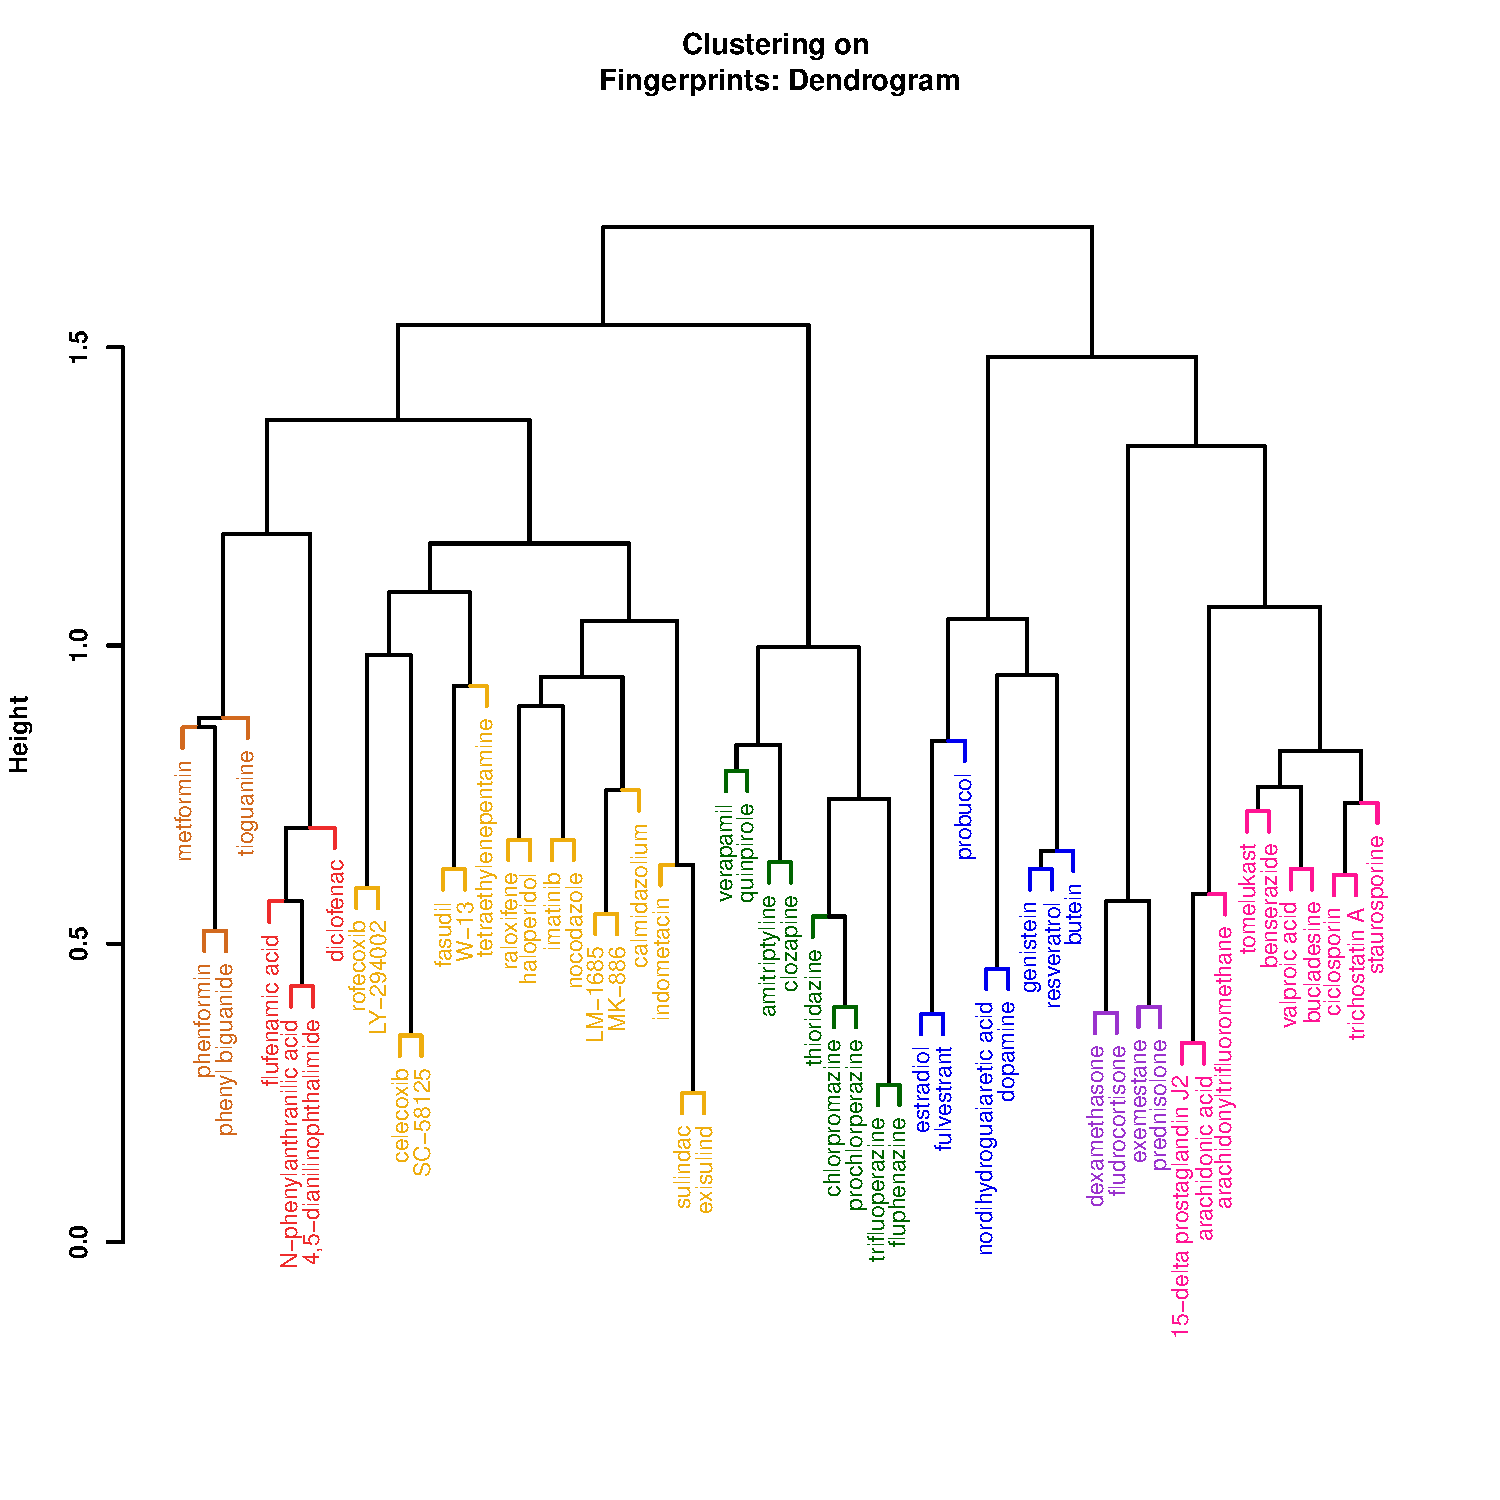
\includegraphics{IntClustVignette-ClusterPlotF}
\caption{{\it FP - MCF7}\label{MCF7_F}}
\end{minipage}%
  \begin{minipage}[b]{.5\linewidth}
     \centering
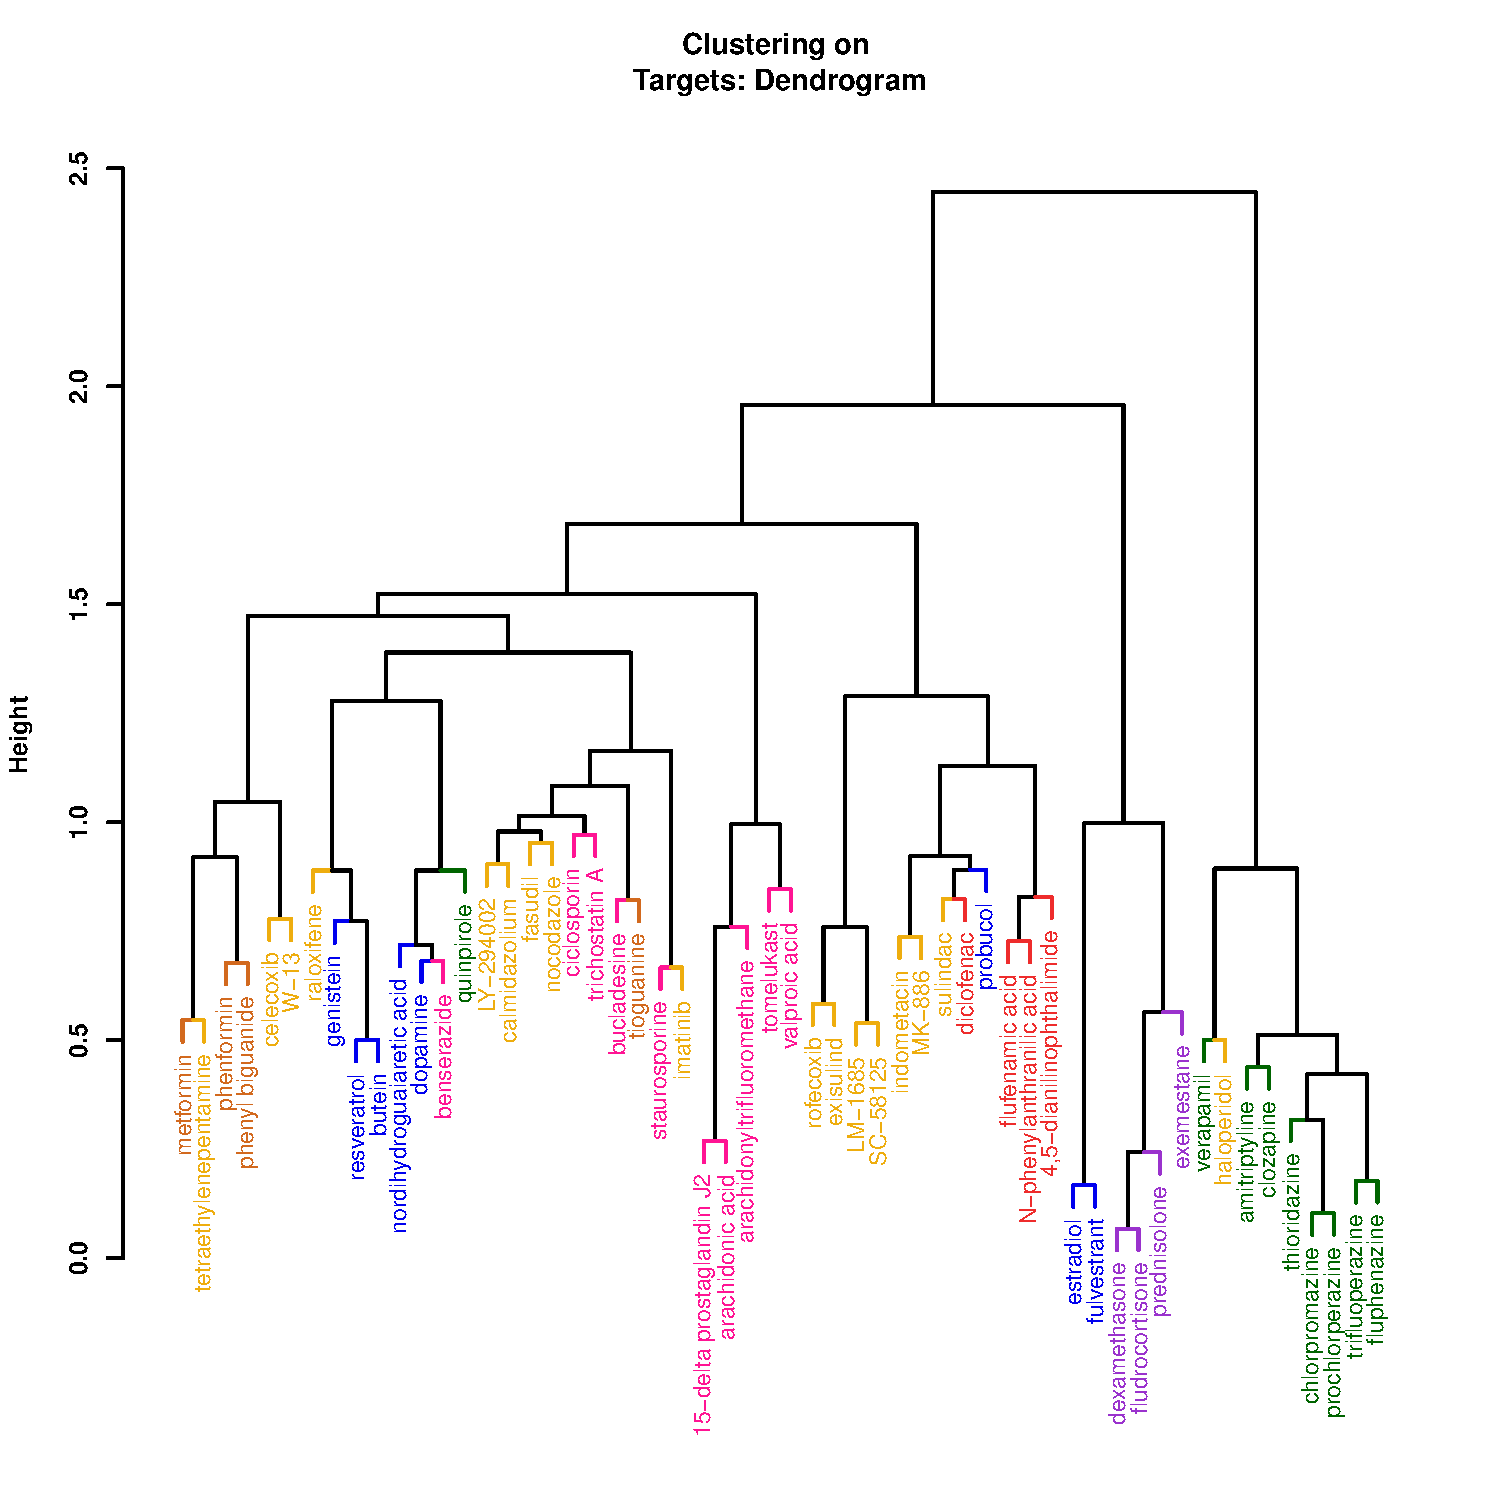
\includegraphics{IntClustVignette-ClusterPlotT}
\caption{{\it TP - MCF7}\label{MCF7_T}}
 \end{minipage}
\end{figure}
\noindent Figure \ref{MCF7_F} on the left is the results of the fingerprint
clustering of the MCF7 data colored by the result of the fingerprint clustering.
This implies that the dendrogram was cut into $7$ clusters and each cluster was
given a color. On the right in figure \ref{MCF7_T} the result of the target prediction
clustering is depicted. The dendrogram was also cut into $7$ clusters but each
leaf (each compound) was given the same color it had in the fingerprint
clustering to make a comparison possible. We could for example investigate the
green cluster determined by figure \ref{MCF7_F}. It is seen that in figure
\ref{MCF7_T} the cluster does not undergo a lot of changes under the influence
of the target predicions. The group is reformed but one compound has dissapeared
and has been replaced by a compound of the what was the yellow cluster in figure
\ref{MCF7_F}.
\subsection{Multi-Source Clustering}
Several multi-source clustering procedures have been implemented in the IntClust
package. A brief overview is provided here.
\subsubsection{Aggregated Data Clustering (ADC)}
Aggregated data clustering can only be applied if all data sources are of the
same type. This is because the first step is to fuse all data matrices into one
larger matrix such that in the end only one data matrix remains. Next,
clustering is performed on this single matrix.
\begin{Schunk}
\begin{Sinput}
> L=list(fingerprintMat,targetMat)
> MCF7_ADC=ADC(List=L,distmeasure="tanimoto",normalize=FALSE,method=NULL,
              clust="agnes", linkage="ward")
\end{Sinput}
\end{Schunk}
\subsubsection{Aggregated Data Ensemble Clustering (ADEC)}
Aggregated data ensemble clustering starts as ADC with the
fusion of the data matrices and can thus only be performed if all data matrices
are of the same type. Then ensemble clustering is performed on the fused data
matrix. This comes down to repeatedly applying hierarchical clustering. The
original version of the method (\cite{Fodeh2013}) is implemented as version
ADECa and two adaptions were made as ADECb and ADECc. A more detailed
explanation follows.\\ \\
Call $m$ the number of features of the fused data matrix $A$.
\begin{enumerate}
\item In every iteration, a random sample of features $r$ of $A$ is taken and
form matrix $A$'. The number of features is randomly set between $\frac{m}{2}$
and $m-1$ each time.
\item Hierarchical clustering is performed on $A$'. The dendrogram is cut into a
specific number of clusters $k$.
\item The incidence matrix $C$ is computed. This binary matrix has as rows and
columns the objects of the data set. A value of $0$ indicates that these
objects belong to the same cluster while $1$ implies that they do not. This
seems counterintuitive but was done to ensure distances rather than
similarities.
\item The co-association matrix $S$ is iteratively computed as
$$S^{(t+1)}=S^{(t)}+C$$ and indicates the number of times a pair of objects
belong to the same cluster.
\item The steps in 1-4 are repeated $t$ times.
\item Finally, hierarchical clustering is performed on the resulting
co-association matrix $S$ which yields the result of the ensemble clustering.
\end{enumerate}
\noindent This is the description of ADECa. In version b a random sample of
features will not be taken but instead all features will be used in every
iteration. Variation is ensured by cutting the resulting dendrogram multiple
times for a range of values for $k$. Version c is a combination of version a and
b. Every iteration a random sample of features will be taken and each resulting
dendrogram will be cut into cluster several times for a range of values for $k$.
\begin{Schunk}
\begin{Sinput}
> L=list(fingerprintMat,targetMat)
> MCF7_ADECa=ADECa(List=L,distmeasure="tanimoto",normalize=FALSE,method=NULL,
                  t=20,r=NULL,nrclusters=7,clust="agnes",linkage="ward")
> MCF7_ADECb=ADECb(List=L,distmeasure="tanimoto",normalize=FALSE,method=NULL,
                  nrclusters=seq(5,25,1),clust="agnes",linkage="ward")
> MCF7_ADECc=ADECc(List=L,distmeasure="tanimoto",normalize=FALSE,method=NULL,
                  t=20,r=NULL, nrclusters=seq(5,25),clust="agnes",linkage="ward")
\end{Sinput}
\end{Schunk}
\subsubsection{Complementary Ensemble Clustering (CEC)}
Complementary ensemble clustering (\cite{Fodeh2013})
shows similarities with ADEC. Instead of merging the data matrices, ensemble
clustering is performed on each data matrix separately as described for ADEC.
After the iterative procedure, the co-association matrices are combined via a
weigted linear combination into a final weigted co-association matrix. On this
final matrix clustering is performed once more which yields the final result.
The version CECa, CECb and CECc differ respectively from each other as where
ADECa, ADECb and ADECc differ.
\begin{Schunk}
\begin{Sinput}
> L=list(fingerprintMat,targetMat)
> MCF7_CECa=CECa(List=L,distmeasure=c("tanimoto","tanimoto"),normalize=FALSE,
                method=NULL,t=20,r=NULL,nrclusters=c(7,7),clust="agnes",
                linkage="ward",StopRange=FALSE)
> MCF7_CECb=CECb(List=L,distmeasure=c("tanimoto","tanimoto"),normalize=FALSE,
                method=NULL,nrclusters=seq(5,25,1),clust="agnes",
                linkage="ward",StopRange=FALSE) 
> MCF7_CECc=CECc(List=L,distmeasure=c("tanimoto","tanimoto"),normalize=FALSE,
                method=NULL,t=20,r=NULL,nrclusters=seq(5,25),clust="agnes",
                linkage="ward",StopRange=FALSE)		 
\end{Sinput}
\end{Schunk}
\subsubsection{Similarity Network Fusion (SNF)}
Similarity network fusion (\cite{Wang2014}) consists of two stages and results
in a sharing of information over all available data sources.
\paragraph{Stage I - The initial step}
A similarity network is set up for each data matrix. First, the distances
between the objects are calculated. These are then rescaled to similarities
relying on the kernel of normal distribution. This results in a matrix with a
similarity value for each pair of objects. The similar objects were
found, the higher their similarity value. The connection to a network is made
when the matrix is visualized as weighted graph with the objects as nodes and
the pairwise similarities as weights on the edges. 
\paragraph{Stage II - The network fusion step}
To perform a fusion of the networks, two more matrices are necessary. The first
is a normalized version of the similarity matrix and is referred to as a global
matrix. The second is also a normalized version of the similarity matrix but
only considers the points in the vicinity of objects. This implies that the
normalization is performed for a specific number of neighbours and all other
values in the row are set to $0$. This matrix is called the local matrix. The assumption is
that objects in the neighbourhood bring more reliable information forward
than objects further away. Each global matrix is now updated via a matrix
multiplication of the corresponding local matrices and the average of all other
global matrices. After a number of iterations, the average of the updated global
matrices is taken as the final fused network. The similarities are converted to
distances and a final clustering is performed.\\ \\
The R package \texttt{SNFtool} accompagnies the paper by \cite{Wang2014}.
Its functions are combined into SNFa. However, it was noticed that the functions 
do not coincide with the method described in the paper. Therefore SNFb was
written which performs the steps as these were outlined. Versions SNFc shows a
high degree of similarity with version b but instead of performing the
normalization of the local matrix separately, the local matrix is taken as a
submatrix of the global matrix.
\begin{Schunk}
\begin{Sinput}
> L=list(fingerprintMat,targetMat)
> MCF7_SNFa=SNFa(List=L,type="data",distmeasure=c("tanimoto","tanimoto"),normalize=FALSE,
                method=NULL,NN=5,mu=0.5,T=20,clust="agnes",linkage="ward",StopRange=FALSE)
> MCF7_SNFb=SNFb(List=L,type="data",distmeasure=c("tanimoto","tanimoto"),normalize=FALSE,
                method=NULL,NN=10,mu=0.5,T=20,clust="agnes",linkage="ward",StopRange=FALSE)
> MCF7_SNFc=SNFc(List=L,type="data",distmeasure=c("tanimoto","tanimoto"),normalize=FALSE,
                method=NULL,NN=10,mu=0.5,T=20,clust="agnes",linkage="ward",StopRange=FALSE)	   
\end{Sinput}
\end{Schunk}
\subsubsection{Weighted Clustering (WeightedClust)}
Weighted clustering is a straigtforward method. From each data matrix, a
distance matrix ic calculated. The distance matrices are than combined via a
weighted linear combination into one weighted distance matrix on which
clustering is performed.
\begin{Schunk}
\begin{Sinput}
> L=list(fingerprintMat,targetMat)
> MCF7_Weighted=WeightedClust(L,type="data",distmeasure=c("tanimoto","tanimoto"),
                             normalize=FALSE,method=NULL,weight=seq(0,1,0.1),
                             WeightClust=0.5,clust="agnes",linkage="ward",
                             StopRange=FALSE)
\end{Sinput}
\end{Schunk}
\subsubsection{Weighted Similarity Clustering (WeightedSim)}
Weighted similarity clustering (\cite{Perualila-Tan2015}) is practically the
same as weighted clustering but an optimal weight is determined first. Each
single source clustering is compared to every weighted clustering and the
jaccard index is calculated as a representative of their similarity. For every
weight combination, each pair of jaccard indices is compared to each other by
takin their ratios. The weight combinations for which the ratios is closests to
$1$ is taken as the optimal combination.
\begin{Schunk}
\begin{Sinput}
> L=list(fingerprintMat,targetMat)
> MCF7_Weight=DetermineWeight_SimClust(List=L,type="data",weight=seq(1,0,by=-0.01),
                                      nrclusters=7,distmeasure=c("tanimoto","tanimoto"),
                                      normalize=FALSE,method=NULL,clust="agnes",
                                      linkage="ward",gap=FALSE, maxK=50,
                                      names=c("FP","TP"),StopRange=FALSE,
                                      plottype="sweave",location=NULL)
> L=list(MCF7_F,MCF7_T)	
> MCF7_WeightedSim=WeightedSimClust(List=L,type="clusters",weight=MCF7_Weight$Weight,
                                   clust="agnes",linkage="ward",distmeasure=
                                   c("tanimoto","tanimoto"),normalize=FALSE,
                                   method=NULL,gap=FALSE,maxK=50,nrclusters=7,
                                   names=c("FP","TP"),AllClusters=FALSE,StopRange=FALSE)
\end{Sinput}
\end{Schunk}
\noindent An optimal weight can alternatively be determined by the function
{\it DetermineWeight\_SilClust}. For each provdided weight, the distance
matrices are combined in a weighted combination and medoid clustering with the
{\it pam} function is performed. Based on the silhouette widths and the
cluster membership an optimal weight is determined. See the helpfiles for more details.
\begin{Schunk}
\begin{Sinput}
> L=list(fingerprintMat,targetMat)
> MCF7_Weight=DetermineWeight_SilClust(List=L,type="data",weight=seq(0,1,by=0.01),
                                      distmeasure=c("tanimoto","tanimoto"),
                                      normalize=FALSE,nrclusters=7,names=c("FP","TP"),
                                      nboot=1000,StopRange=FALSE,
                                      plottype="sweave",location=NULL)
\end{Sinput}
\end{Schunk}
\subsubsection{Weighting on Membership Clustering (WonM)}
Weighting on membership performs hierarchical clustering on each data source
separately. With $k$ the number of clusters, the resulting dendrograms
are cut into clusters for a range of values for $k$. Each time, an incidence
matrix is set up. This is a matrix with as rows and columns the objects of the
data set. Its values are $0$ and $1$ with $0$ indicating that a pair of object
resides in the same cluster to ensure distances. The incidence matrices are
first summed over all values of $k$ per data source and then these of the
different data sources are added as well. On the resulting consensus matrix,
hierarchical clustering is performed once again to obtain the final clustering
taking into account information of all data sources.
\begin{Schunk}
\begin{Sinput}
> L=list(fingerprintMat,targetMat)
> MCF7_WonM=WonM(List=L,type="data",distmeasure=c("tanimoto","tanimoto"),
                normalize=FALSE,method=NULL,nrclusters=seq(5,25),clust="agnes",
                linkage="ward",StopRange=FALSE)
\end{Sinput}
\end{Schunk}

\subsection{Comparison of the results}
The clusters of the multi-source methods consist of objects that
are similar on multiple layers of the underlying biology represented by the
multiple data sources. The interest lies in those clusters that remain stable over
the applied methods. If a cluster does not undergo too many changes and is found
multiple times, confidence can be put into those objects belonging together.
Further, it can be hypothesized that the used data sources are related for those
clusters. This can provide more insight into the mechanism of action of the
compounds.\\ \\
A comparison of the results is not done on sight. Different methods cluster the
compounds in a different order and this results in non-corresponding cluster
numbers. Therefore, it was decided to take one method as reference and rearrange
the cluster numbers of the other results to this reference. The re-appointing of
the cluster numbers is based on finding the cluster that relatively has the most
in common with one of the reference clusters and taking over this number. The
function {\it MatrixFunction} was written for this purpose and its algorithm is
partly based on the Gale- Shapley algorithm (\cite{Kleinberg2005})..
It creates a matrix of which the columns are the compounds in the order of
clustering by reference method. The rows are the different methods and the
values of the cells are the rearranged cluster numbers. If each value is
associated with a colour, a visualization of the matrix can be made. A
similarity measure is handy for the comparison of multiple methods. Given a
method to be used as reference, it is observed which compounds are residing in
the same cluster for a second method after applying {\it MatrixFunction}. The
number of compounds that belong to the same cluster is summed and divided by the
total number of objects in the data set. This is computed by the {\it
SimilarityMeasure} function.\\ \\
The {\it MatrixFunction} and {\it SimilarityMeasure} functions are combined in
the {\it ComparePlot} function. 
\begin{Schunk}
\begin{Sinput}
> L=list(MCF7_F,MCF7_ADC,MCF7_ADECa,MCF7_ADECb,MCF7_ADECc,MCF7_CECa,MCF7_CECb,
        MCF7_CECc,MCF7_SNFa,MCF7_SNFb,MCF7_SNFc,MCF7_WonM,MCF7_Weighted,
        MCF7_WeightedSim,MCF7_T)
> names=c("FP","ADC","ADECa","ADECb","ADECc","CECa","CECb","CECc","SNFa","SNFb",
         "SNFc","WonM","Weighted","WeightedSim","TP")
\end{Sinput}
\end{Schunk}
\newpage
\begin{figure}[!h] 
\centering
\begin{Schunk}
\begin{Sinput}
> ComparePlot(List=L,nrclusters=7,cols=Colors,fusionsLog=TRUE,WeightClust=TRUE,
             names=names,margins=c(9.1,4.1,4.1,4.1),plottype="sweave",location=NULL)
\end{Sinput}
\end{Schunk}
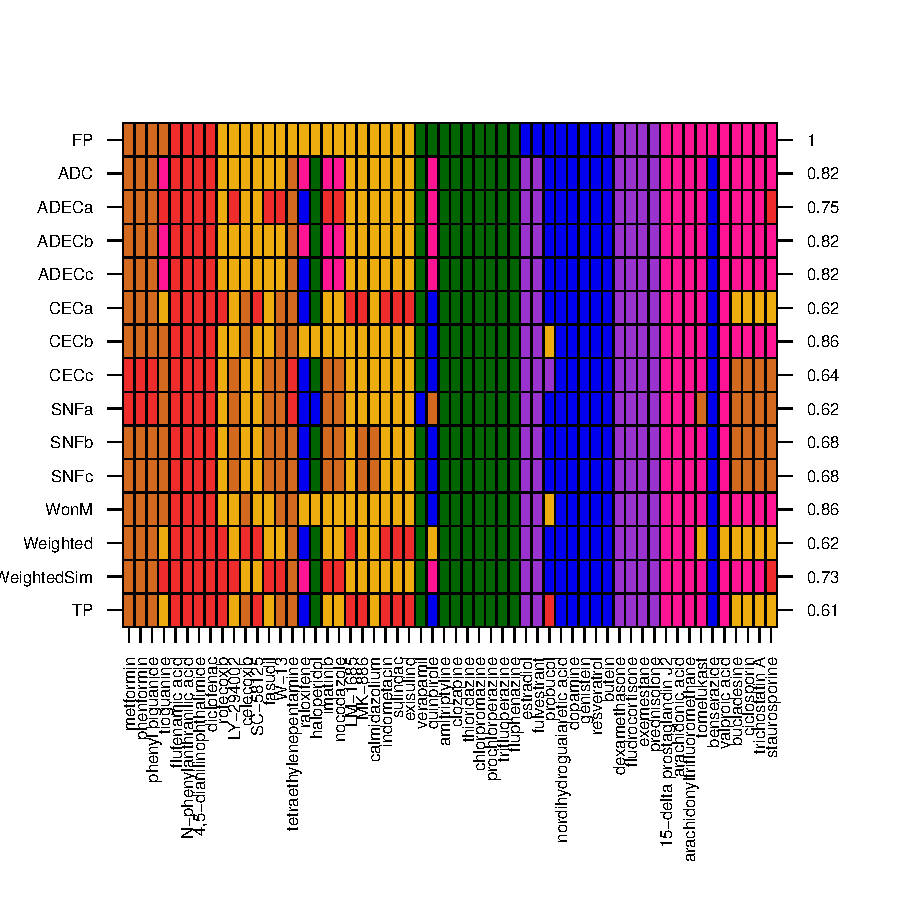
\includegraphics{IntClustVignette-ComparePlot1}
\caption{{\it Comparison of the results for the CMAP MCF7 data}\label{MCF7_All}}
\end{figure}
\noindent Figure \ref{MCF7_All} shows a comparison of all executed clustering
procuderes with the fingerprint clustering as a reference. All other methods were reordered
accordingly. We notice that the green cluster remains stable over all other
methods since all  but one are grouped together every time. Under the influence
of the target predictions one compound dissapears and is replaced by another.
For the weighted procedures, the result for a weight of $0.5$ is shown. This
figure could also have been made over the weights in the weighted clusterings
procedures as presented below.
\begin{Schunk}
\begin{Sinput}
> L=list(MCF7_F,MCF7_Weighted,MCF7_T)
> names=c("FP",seq(1,0,-0.1),"TP")
> 
\end{Sinput}
\end{Schunk}
\newpage
\begin{figure}[!h] 
\centering
\begin{Schunk}
\begin{Sinput}
> ComparePlot(List=L,nrclusters=7,cols=Colors,fusionsLog=TRUE,WeightClust=FALSE,
             names=names,margins=c(9.1,4.1,4.1,4.1),plottype="sweave",location=NULL)
\end{Sinput}
\end{Schunk}
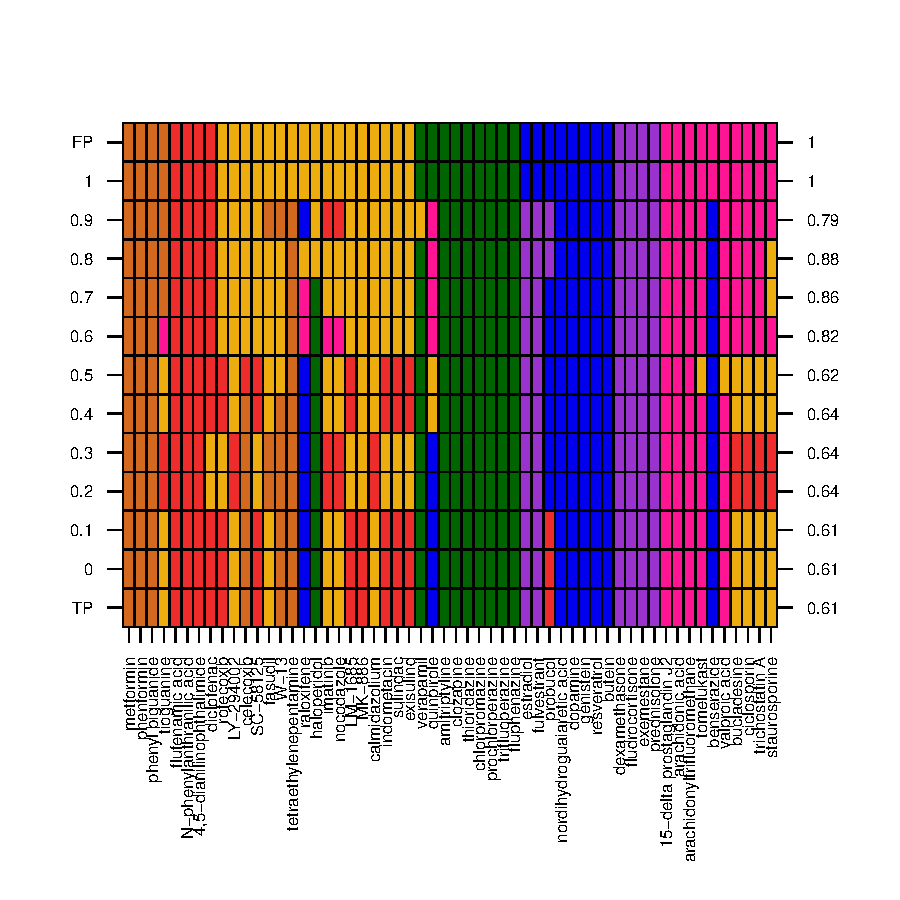
\includegraphics{IntClustVignette-ComparePlot2}
\caption{{\it Comparison of the weights in the weighted clustering for the CMAP
MCF7 data}\label{MCF7_Weights}}
\end{figure}
\noindent It is seen that again, as soon as target prediction information is
involved, one compound dissapears from the cluster while all others remain. For higher
weights, another compound joins the cluster.\\ \\
Further, it is possible to cluster the single source clusterings and
multi-source clustering next to each other such that a visual comparison is
possible. This is mostly interesting of more than $2$ data sources are
available. The function will here be demonstrated for $2$ nonetheless.
It is made sure that for both comparison plots the same reference has been used,
namely the first element of ListM.
\begin{Schunk}
\begin{Sinput}
> LS=list(MCF7_F,MCF7_T)
> LM=list(MCF7_ADC,MCF7_ADECa,MCF7_ADECb,MCF7_ADECc,MCF7_CECa,MCF7_CECb,
 		MCF7_CECc,MCF7_SNFa,MCF7_SNFb,MCF7_SNFc,MCF7_WonM,MCF7_Weighted,
 		MCF7_WeightedSim)
> nS=c("FP","TP")
> nM=c("ADC","ADECa","ADECb","ADECc","CECa","CECb","CECc","SNFa","SNFb",
       "SNFc","WonM","Weighted","WeightedSim")
> CompareSvsM(ListS=LS,ListM=LM,nrclusters=7,cols=Colors,fusionsLogS=TRUE,
             fusionsLogM=TRUE,WeightClustS=TRUE,WeightClustM=TRUE,
             namesS=nS,namesM=nM,margins=c(8.1,3.1,3.1,4.1),plottype="sweave",
             location=NULL)
\end{Sinput}
\end{Schunk}
\begin{figure}[H]  
\centering
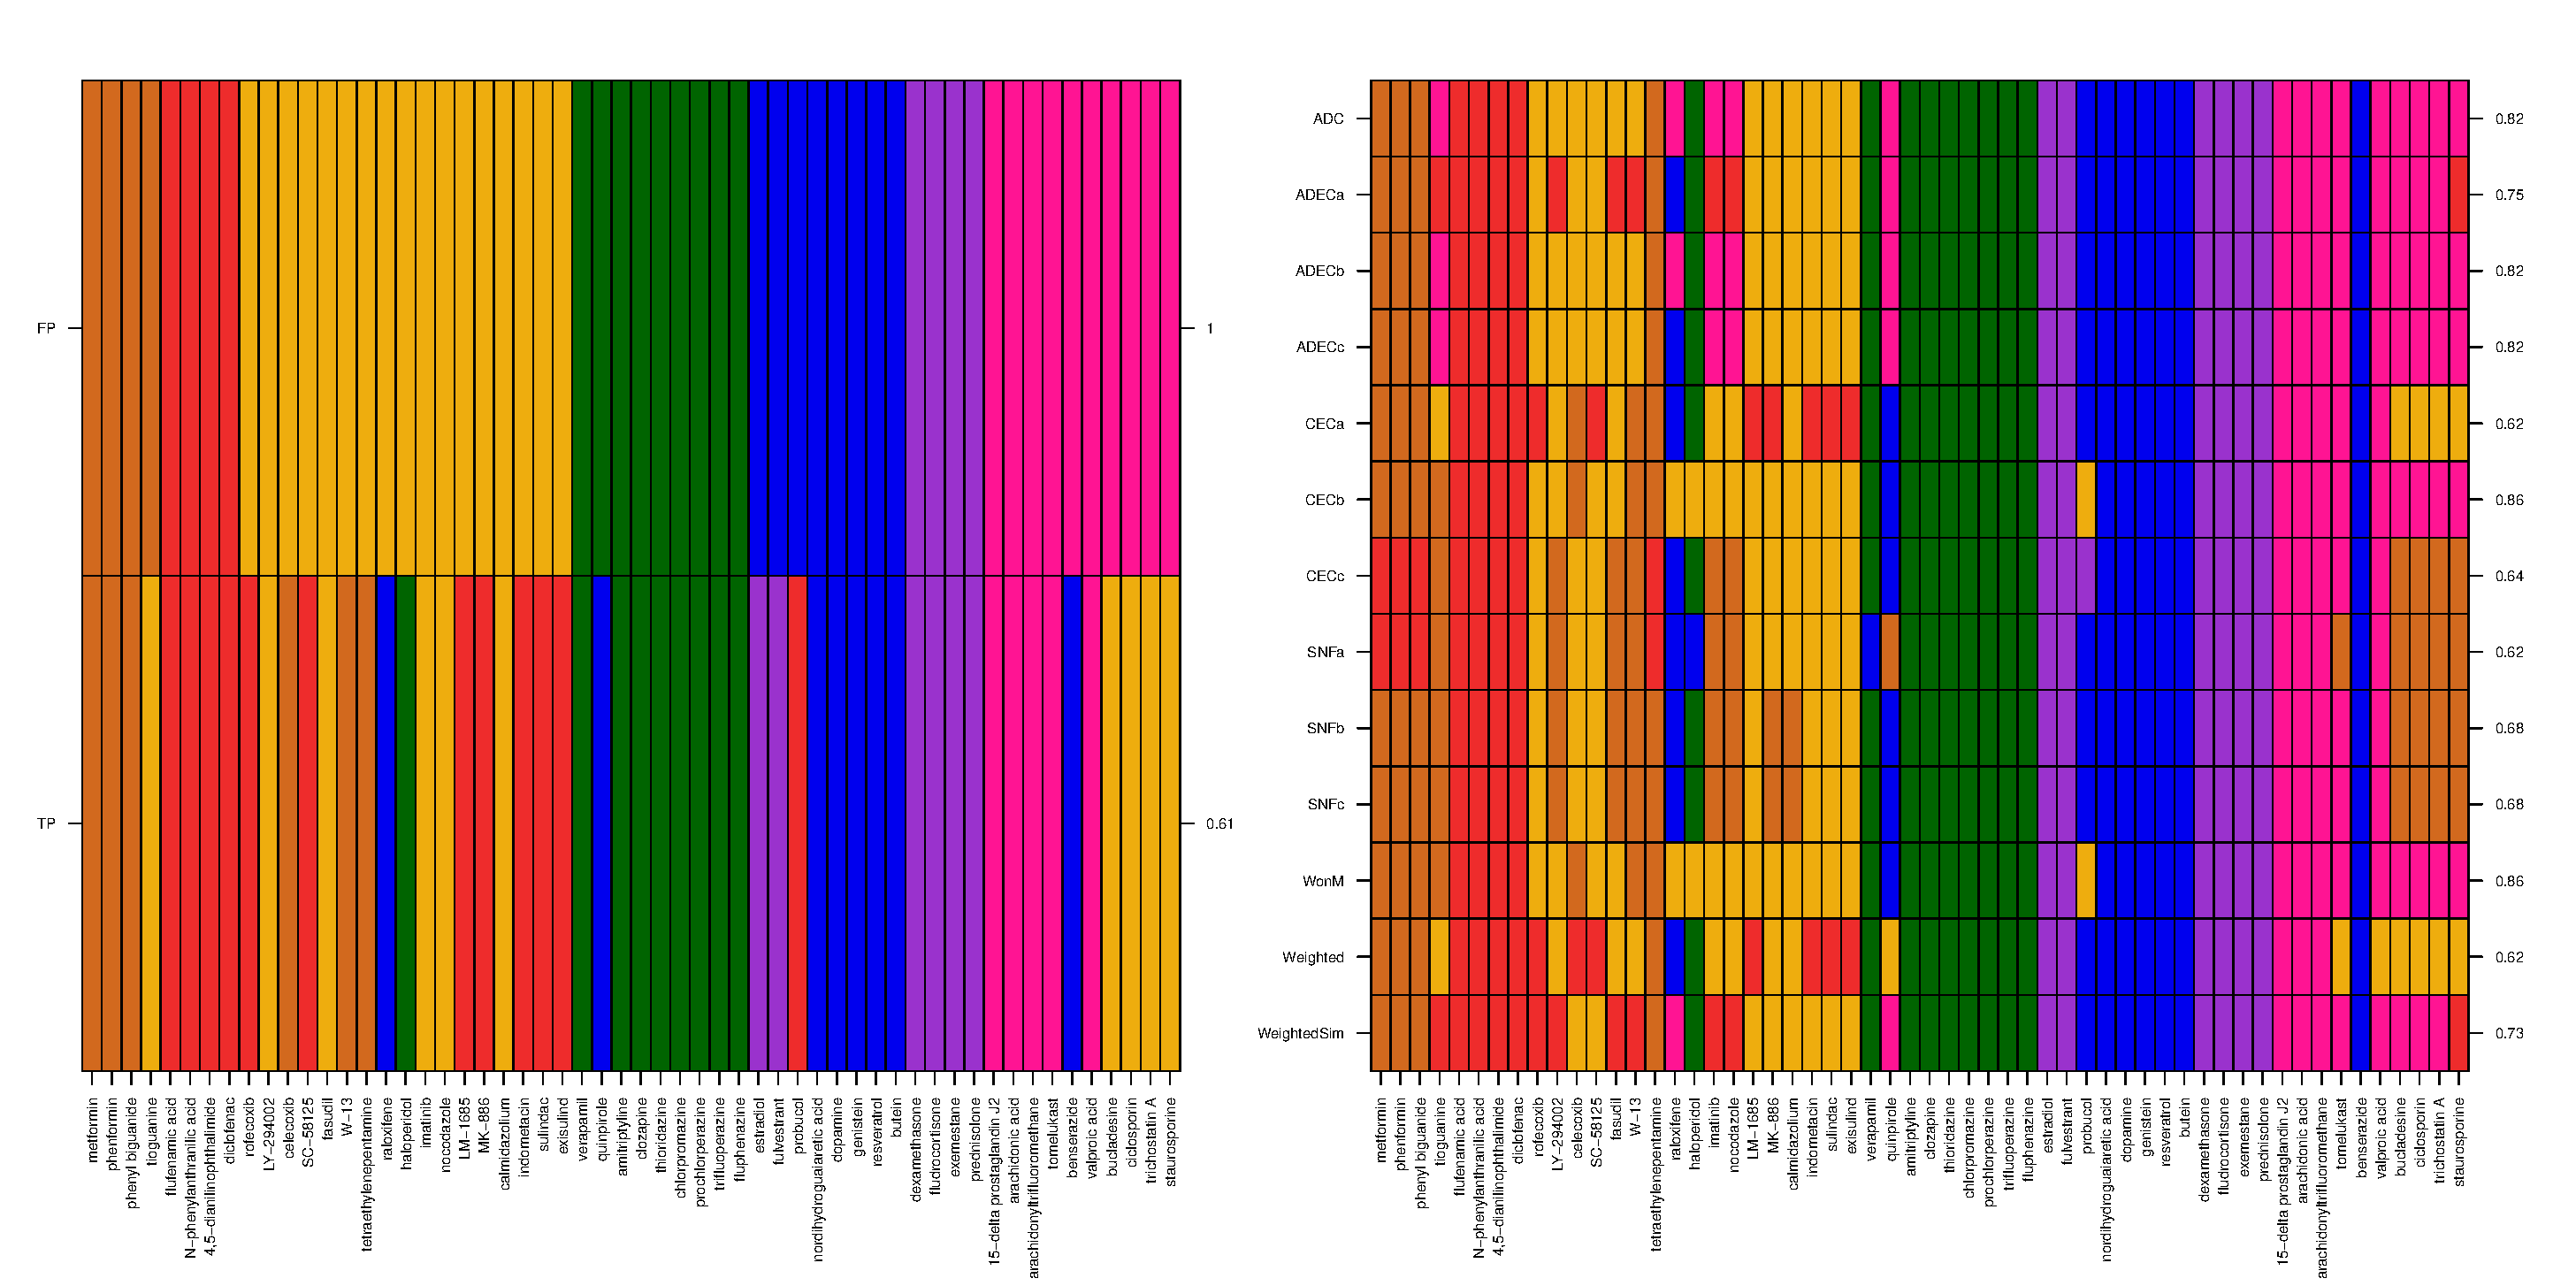
\includegraphics[width=14cm,height=7cm]{CompareSvsM.pdf}
\caption{{\it Comparison of single source and multi-source
clustering}\label{MCF7_SvsM}}
\end{figure}
\noindent Further, an interactive function exists as well. In this function a
comparison plot will be made with the {\it ComparePlot} function of the results
provided in ListM. Then, there exists the opportunity to click on this figure to
either indicate one specific cluster or an entire method. To indicate a cluster,
we click on the color of that cluster for the method of choice. To indicate an
entire method, we click on the name of the method on the left of the figure.
The indicated cluster/method will then be compared to the elements provided in
ListS in a new plot. It is made sure that for both comparison plots the same
reference has been used, namely the first element of ListM.
\begin{Schunk}
\begin{Sinput}
> LS=list(MCF7_F,MCF7_T)
> LM=list(MCF7_ADC,MCF7_ADECa,MCF7_ADECb,MCF7_ADECc,MCF7_CECa,MCF7_CECb,
 		MCF7_CECc,MCF7_SNFa,MCF7_SNFb,MCF7_SNFc,MCF7_WonM,MCF7_Weighted,
 		MCF7_WeightedSim)
> nS=c("FP","TP")
> nM=c("ADC","ADECa","ADECb","ADECc","CECa","CECb","CECc","SNFa","SNFb",
 		"SNFc","WonM","Weighted","WeightedSim")
> Colors=c(Colors,"grey")
> CompareInteractive(ListM=LM,ListS=LS,nrclusters=7,cols=Colors,fusionsLogM=TRUE,
                    fusionsLogS=TRUE,WeightClustM=TRUE,WeightClustS=TRUE,
                    namesM=nM,namesS=nS,marginsM=c(8,4.5,2,2.5),marginsS
                    =c(8,4.5,2,2.5),Interactive=TRUE,N=2)
\end{Sinput}
\end{Schunk}
\newpage
\begin{figure}[H]  
\centering
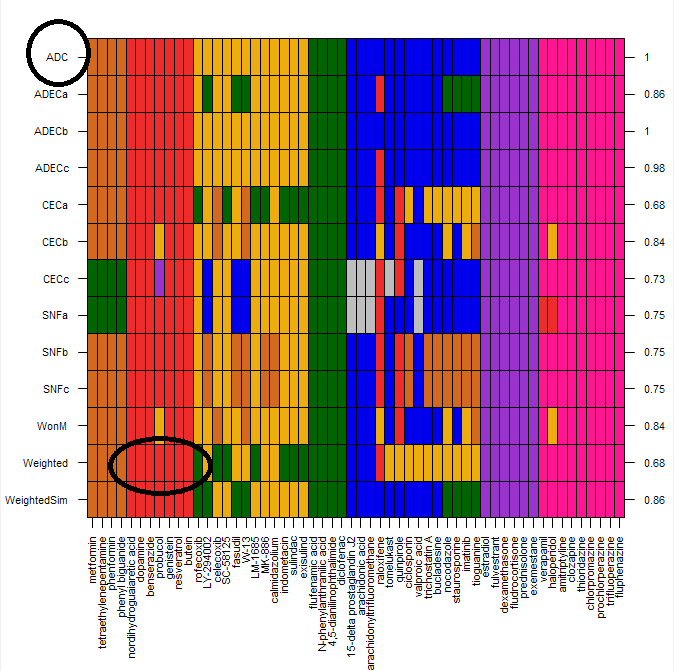
\includegraphics[width=10cm,height=10cm]{Interactive.png}
\end{figure}
\begin{figure}[H]
\begin{minipage}[b]{.5\linewidth}
\centering
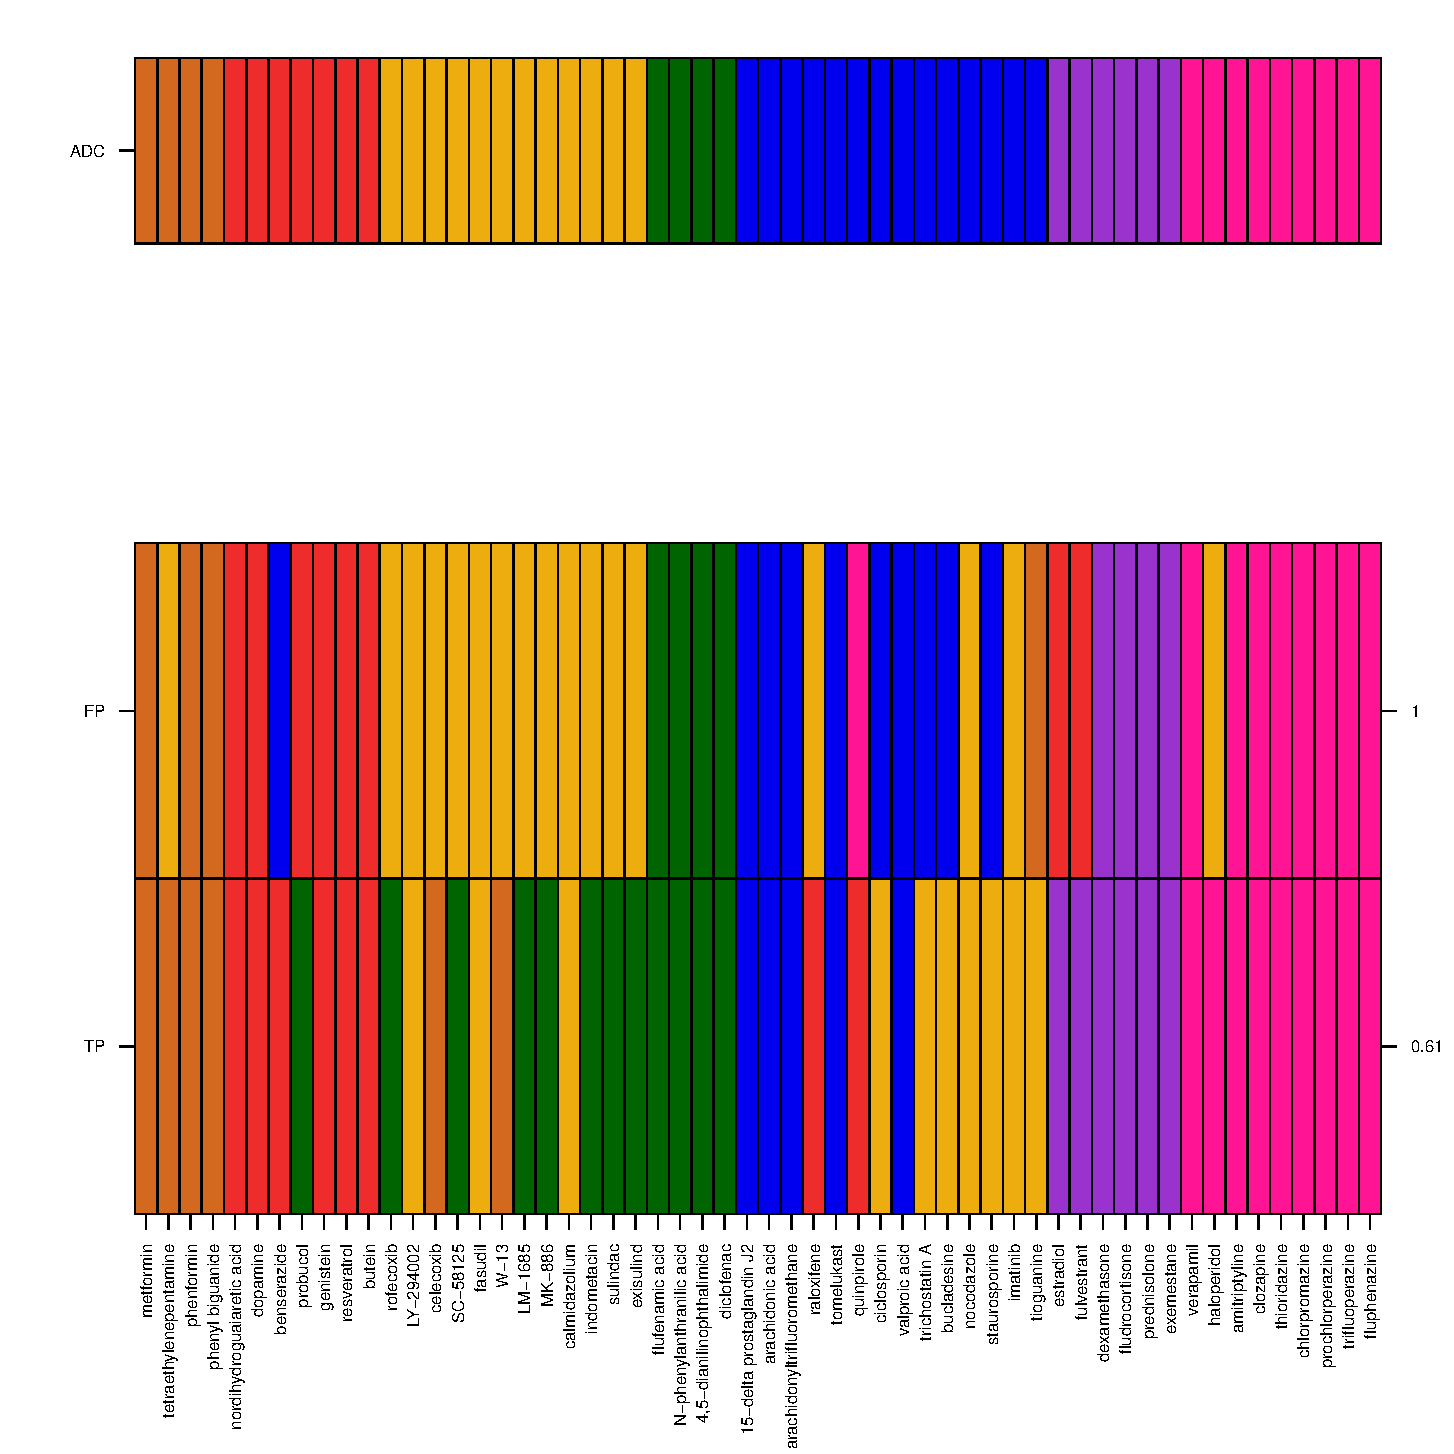
\includegraphics[width=8cm,height=8cm]{InteractiveMethod.pdf}
\end{minipage}%
\begin{minipage}[b]{.5\linewidth}
\centering
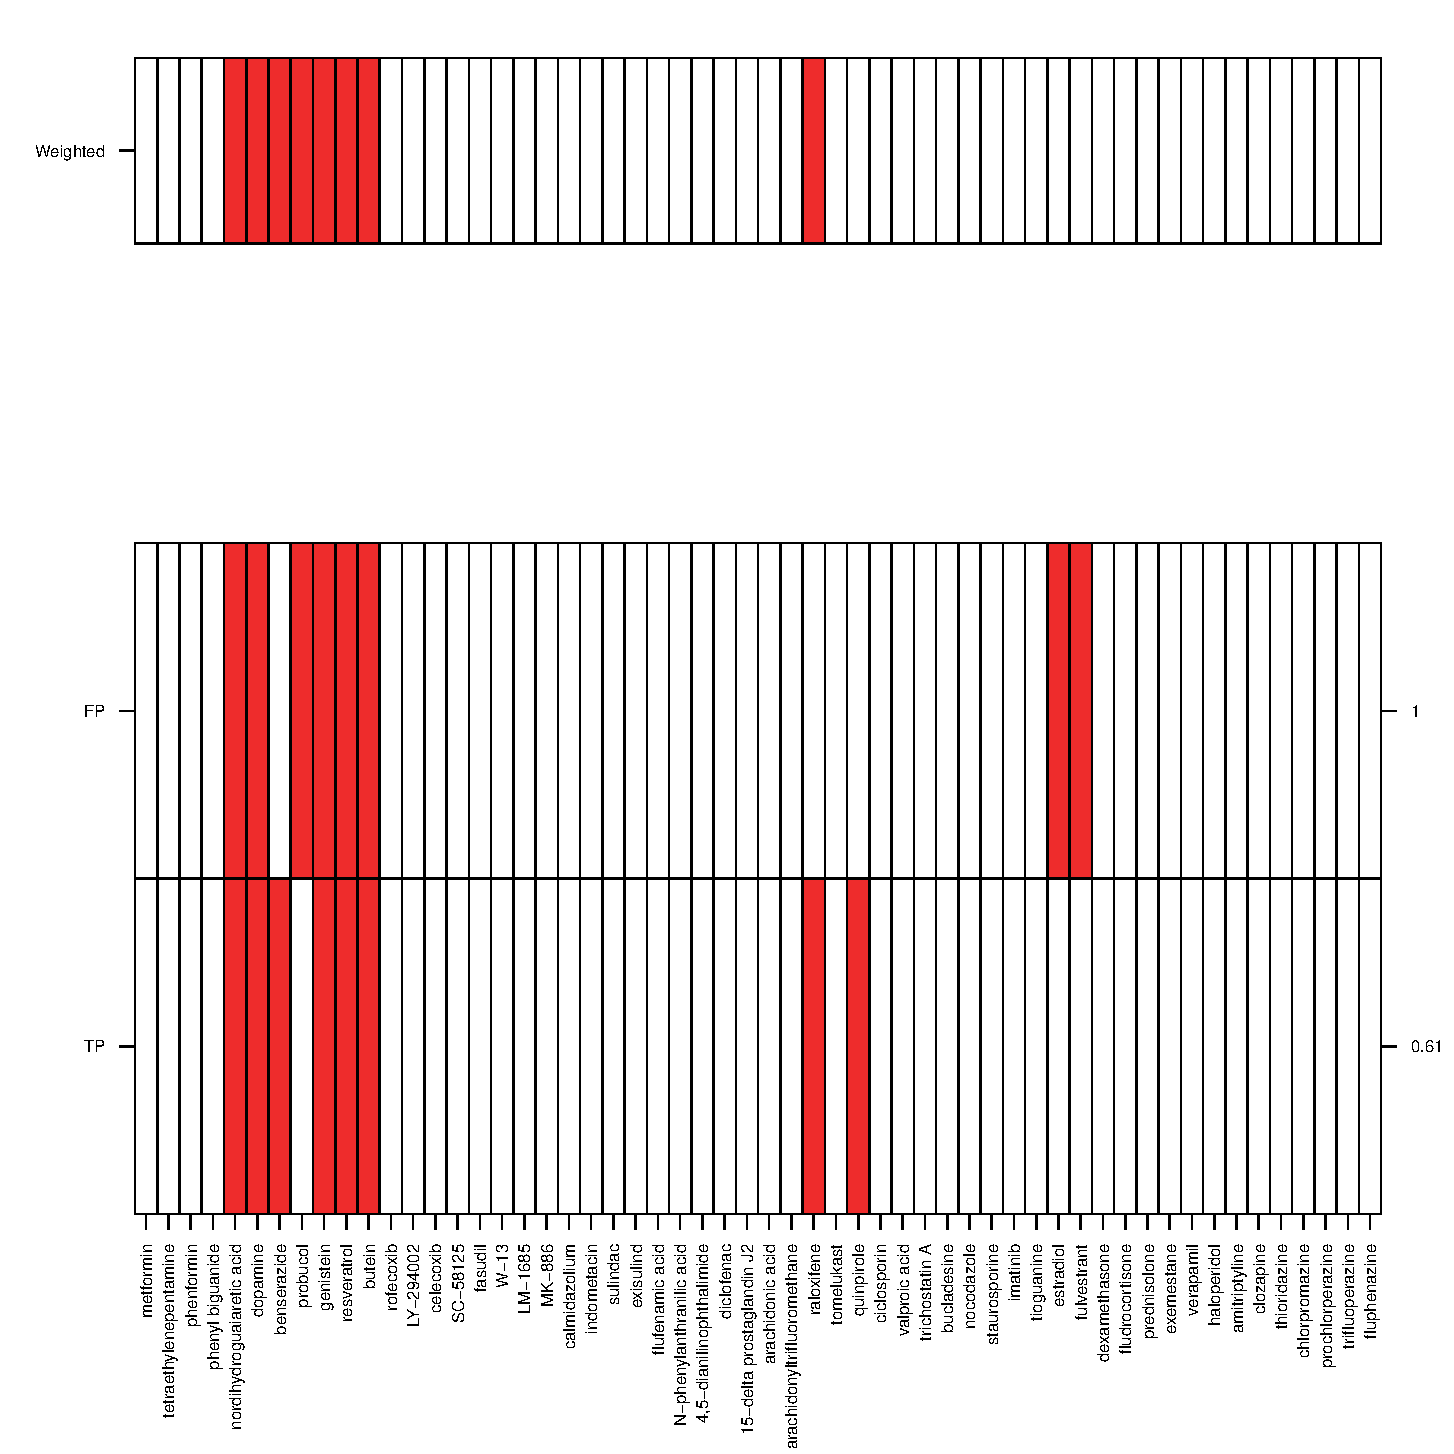
\includegraphics[width=8cm,height=8cm]{InteractiveCluster.pdf}
\end{minipage}
\caption{{\it Interactive Plot - Example}\label{MCF7_Inter}}
\end{figure}
\newpage
\noindent Two clustering results X and Y can be compared with the help of a test
statistic calculated by the \texttt{CompareSilCluster} function. Single data
sources can be provided in their data format. A distance matrix is necessary for
all multiple source clusterings. A medoid clustering is performed of which the
silhouette widths and cluster memberships are retrieved. The silhouette widths
of data X are regressed against the corresponding memberships but also against
the memberships determined by data Y. The $R^{2}$ values are obtained and the
statistic is calculated as:
%$$ S=|\sum{R^2_{XX}}-\sum{R^2_{XY}}|.$$
A p-value is obtained by bootstrapping the distance matrices.
\begin{Schunk}
\begin{Sinput}
> List=list(fingerprintMat,targetMat)
> Comparison=CompareSilCluster(List=List,type="data",distmeasure=c("tanimoto",
                              "tanimoto"),normalize=FALSE,method=NULL,
 		                      nrclusters=7,names=c("FP","TP"),nboot=1000,
                               StopRange=FALSE,plottype="sweave",location=NULL)
> Comparison
\end{Sinput}
\end{Schunk}
\subsection{Selection of a Specific Cluster}
As mentioned above, interest lies in stable clusters. We can now select one
specific cluster and perform further analysis. We investigate of which compounds
the cluster exists and how it was formed over the different results and/or
weights.\\ \\
To find the compounds of a cluster, we can use the {\it FindCluster} function.
Based on the matrix produced by {\it MatrixFunction}, we can proivde the row and
the cluster number (counting from $1$ to $7$ from left to right with every color
being a new cluster in the first row) and the compounds of that cluster will be
returned. We will focus on the green cluster of the target predictions.
\begin{Schunk}
\begin{Sinput}
> L=list(MCF7_F,MCF7_ADC,MCF7_ADECa,MCF7_ADECb,MCF7_ADECc,MCF7_CECa,MCF7_CECb,
        MCF7_CECc,MCF7_SNFa,MCF7_SNFb,MCF7_SNFc,MCF7_WonM,MCF7_Weighted,
        MCF7_WeightedSim,MCF7_T)
> Comps=FindCluster(List=L,nrclusters=7,select=c(15,4))
> Comps
\end{Sinput}
\begin{Soutput}
[1] "haloperidol"      "verapamil"       
[3] "amitriptyline"    "clozapine"       
[5] "thioridazine"     "chlorpromazine"  
[7] "prochlorperazine" "trifluoperazine" 
[9] "fluphenazine"    
\end{Soutput}
\end{Schunk}
Further, we can track how this cluster was formed with the help of the {\it
TrackCluster} function. We will indicate to follow the cluster
specifically (followClust=TRUE) and not the largest group of compounds of the
orginally indicated cluster that remain together (followMaxComps=FALSE). This
might involve a change of cluster.
\begin{Schunk}
\begin{Sinput}
> L=list(MCF7_F,MCF7_ADC,MCF7_ADECa,MCF7_ADECb,MCF7_ADECc,MCF7_CECa,MCF7_CECb,
        MCF7_CECc,MCF7_SNFa,MCF7_SNFb,MCF7_SNFc,MCF7_WonM,MCF7_Weighted,
        MCF7_WeightedSim,MCF7_T)
> names=c("FP","ADC","ADECa","ADECb","ADECc","CECa","CECb","CECc","SNFa","SNFb",
 		"SNFc","WonM","Weighted","WeightedSim","TP")
> Tracking=TrackCluster(List=L,Selection=Comps,nrclusters=7,followMaxComps=FALSE,
                       followClust=TRUE,fusionsLog=TRUE,WeightClust=TRUE,
                       names=names,SelectionPlot=FALSE,Table=FALSE,
                       CompleteSelectionPlot=TRUE,cols=Colors,plottype="sweave",
                       location=NULL)
\end{Sinput}
\end{Schunk}
\vspace{-1.0cm}
\begin{figure}[H]
\centering
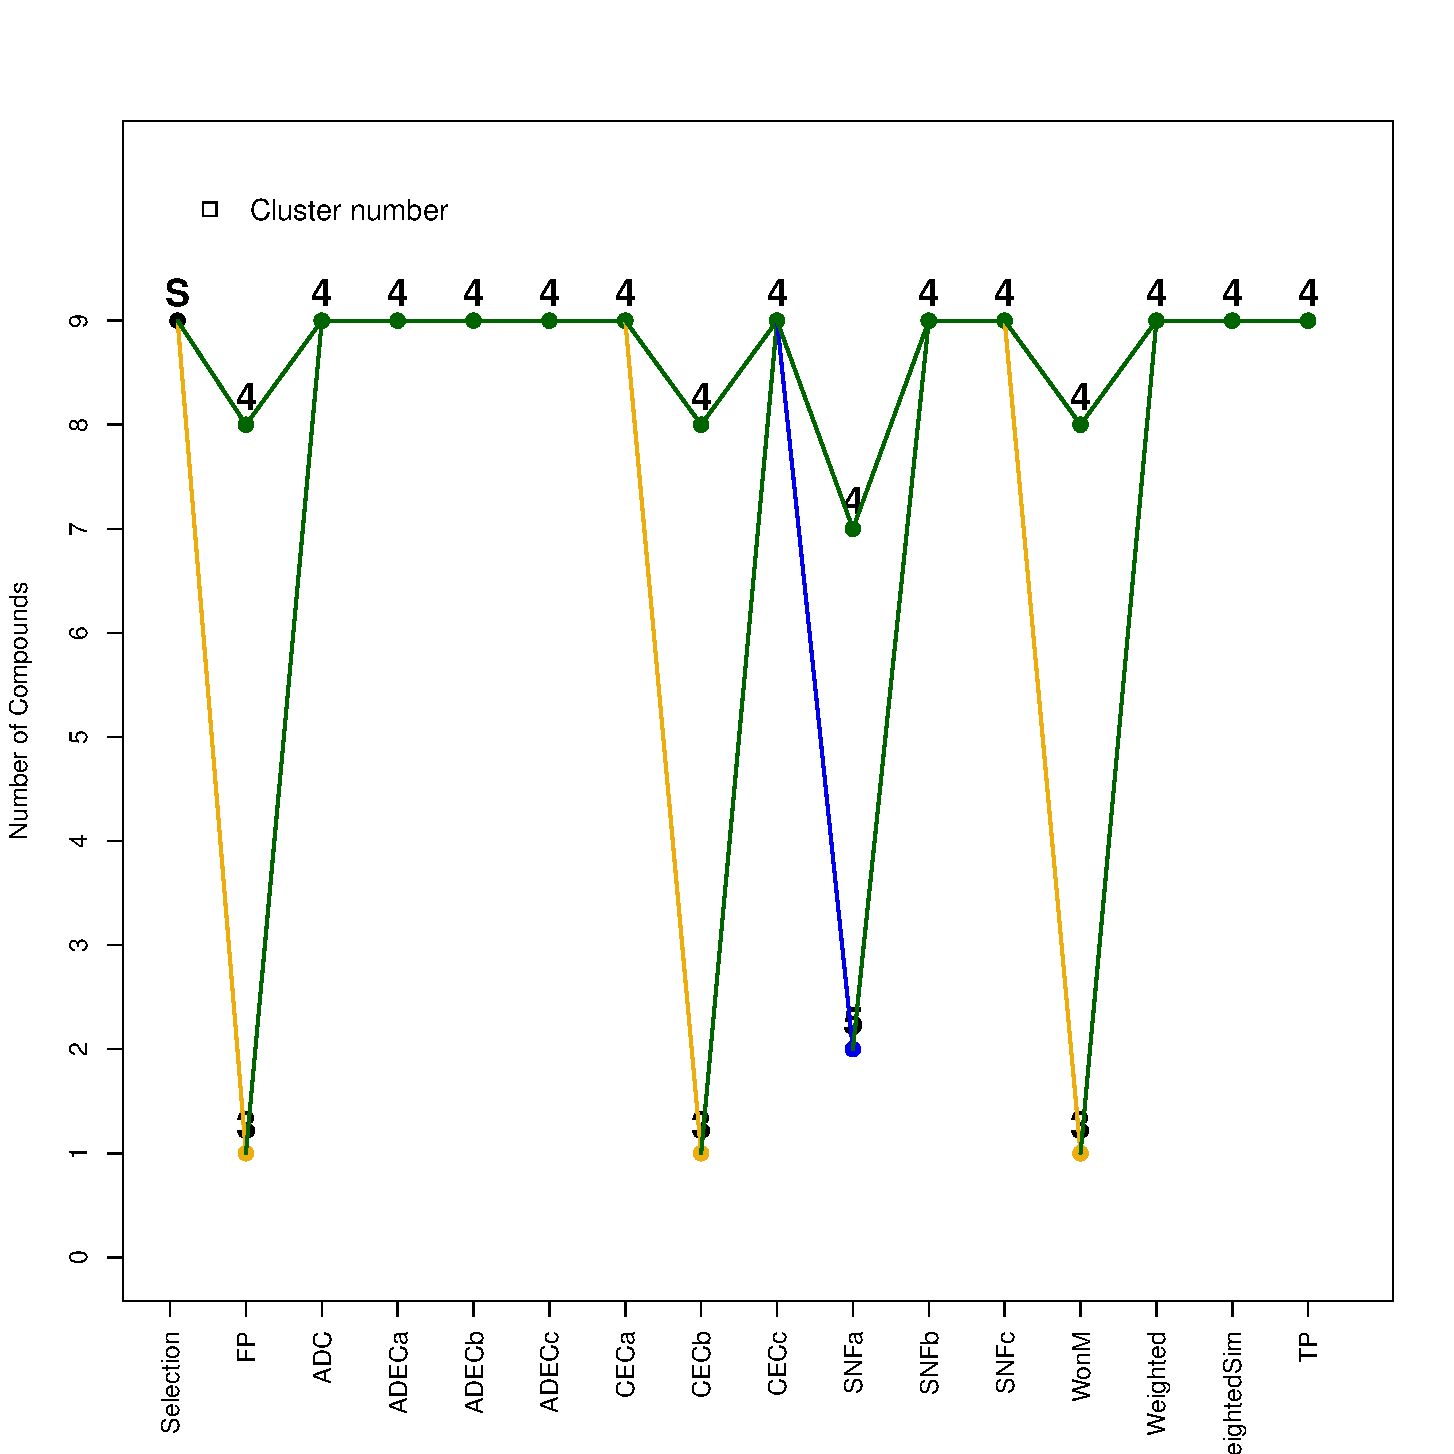
\includegraphics[width=9cm,height=9cm]{Tracking.pdf}
\caption{{\it Tracking of the green cluster over the
methods}\label{MCF7_Track}}
\end{figure}
\noindent A selection of a specific cluster can also be made by inspecting the
heatmap of the similarity values. The function \it{SimilarityHeatmap} plots the
similarity values among the compounds. The input can be a clustering results but
just as well the data source itself. The option to set a cutoff value is
provided. This way, one can but all values below a certain similarity cutoff to
0 while keeping the other values. A more clearer heatmap will the result.
We will draw here the similarity heatmap of the weighted clustering result for
a weight of $0.5$.
\begin{Schunk}
\begin{Sinput}
> SimilarityHeatmap(Data=MCF7_Weighted$Clust,type="clust",distmeasure="tanimoto",
                   normalize=FALSE,method="Q",cutoff=0.90,percentile=TRUE
                   ,plottype="sweave",location=NULL)
> 	
\end{Sinput}
\end{Schunk}
\vspace{-1.0cm}
\begin{figure}[H]
\centering
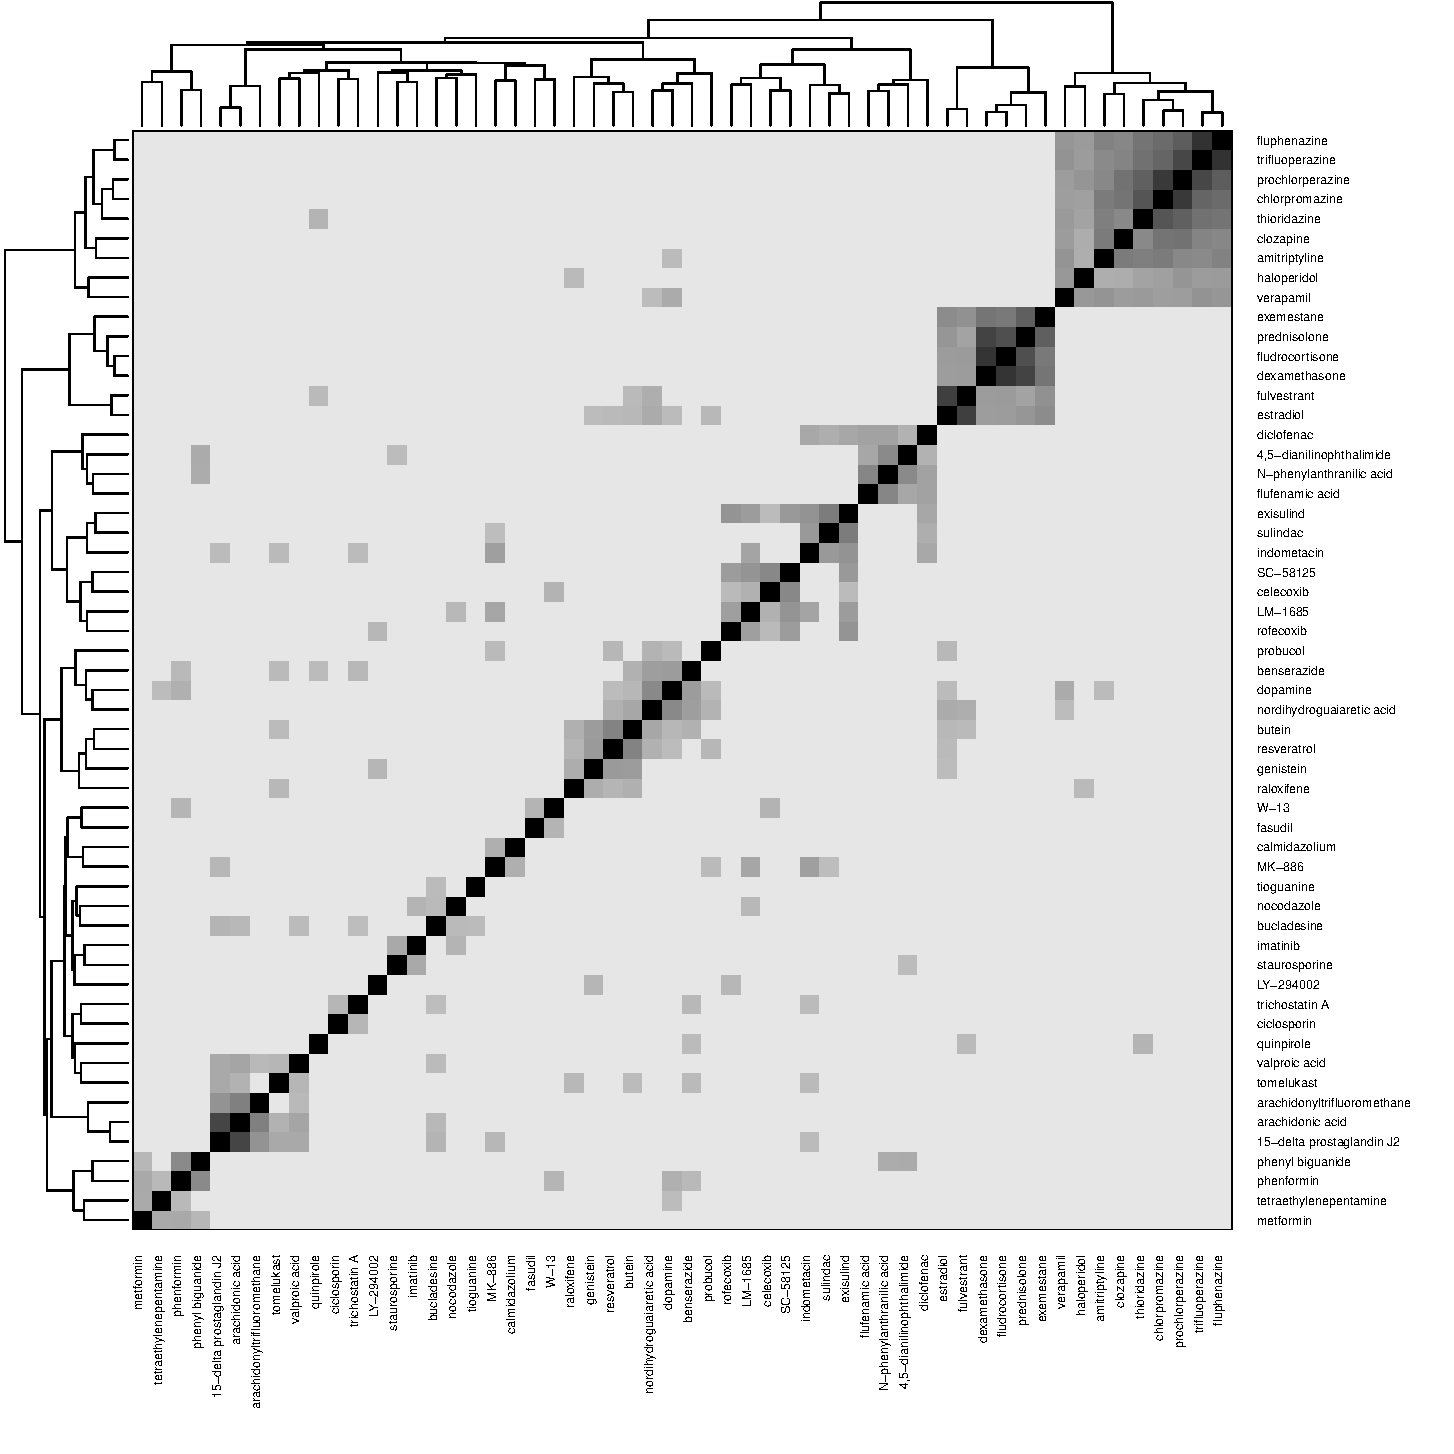
\includegraphics[width=9cm,height=9cm]{SimilarityHeatmap_MCF7W.pdf}
\caption{{\it Similarity Heatmap of the Weighted
Clustering Result.}\label{SimMap}}
\end{figure}
\noindent An experimental function was written to select a group of compounds
directly from a heatmap. The function \it{HeatmapSelection} draws the same
heatmap as shown above but without the dendrograms at the side. The user is now
free to select two points on the heatmap. It is advised that these two points
are in opposite corners of a square that indicates a high similarity among the
compounds. The points do not have to be the exact corners of the group of
interest, a little deviation is allowed as rows and columns of the selected
subset of the matrix with sum equal to 1 are filtered out. A sum equal to one,
implies that the compound is only similar to itself. The function is meant to be
explorative but is experimental. The goal was to make the selection of
interesting compounds easier as sometimes the labels of the dendrograms are too
distorted to be read. If the figure is exported to a pdf file with an
appropriate width and height, the labels can be become readable again. It will
return the names of the compounds that are in the selected square provided that
these show similarity among each other.
\begin{Schunk}
\begin{Sinput}
> CompsHeat=HeatmapSelection(Data=MCF7_Weighted$Clust$DistM,type="dist",cutoff=0.90,percentile=TRUE,
 dendrogram=MCF7_Weighted$Clust,width=7,height=7)
> CompsHeat
\end{Sinput}
\end{Schunk}
\vspace{-1.0cm}
\begin{figure}[H]
\centering
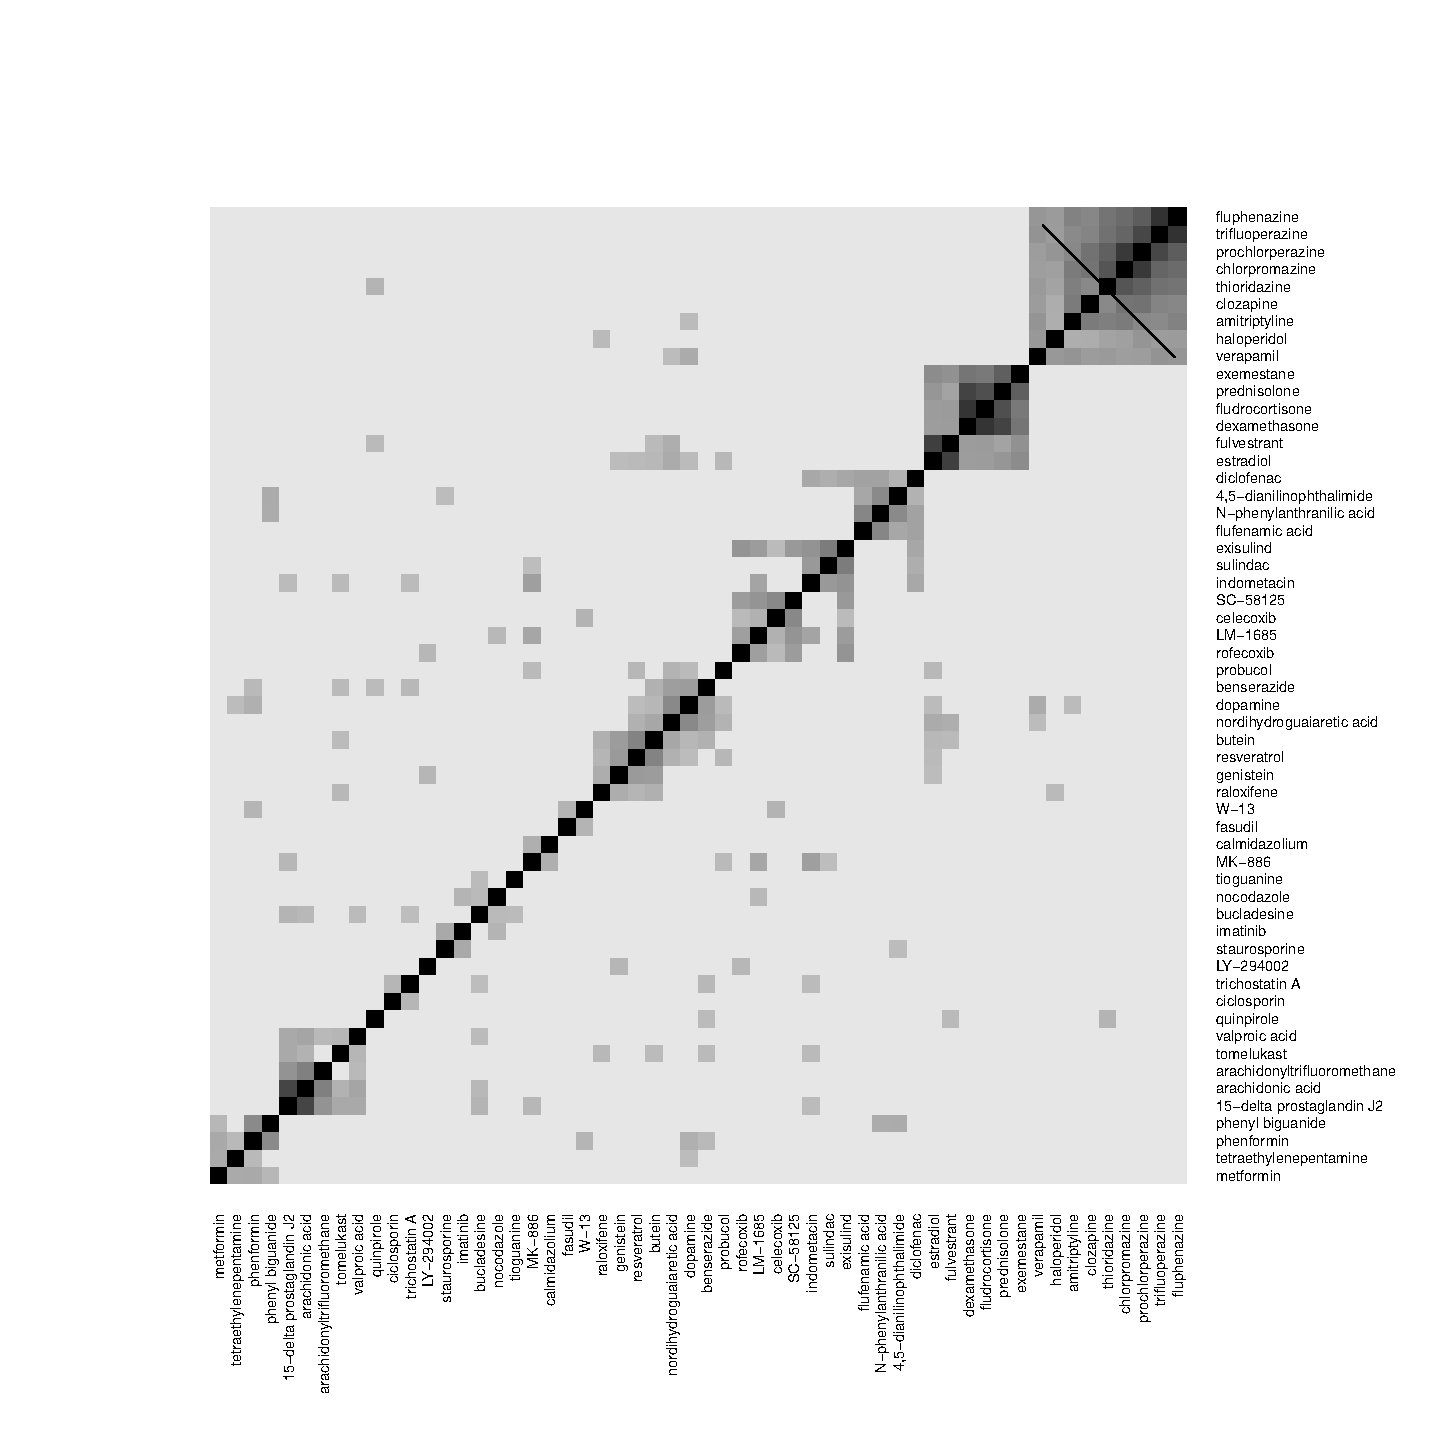
\includegraphics[width=9cm,height=9cm]{HeatmapSelection_MCF7W.pdf}
\caption{{\it Selection of a cluster via the Similarity Heatmap}\label{SimMap}}
\end{figure}
\noindent Next, we perform secondary analysis
on the cluster of interest.
\newpage
\section{Secondary Analysis}
\subsection{Differential Gene Expression}
Interesting genes are those that behave differently in the selected compounds.
The gene may have a higher variation or can be up-regulated or down-regulated.
Several methods exist to find such differentially expressed genes such as a two
sample t-test or a permutation test. It was opted to work with a method called
Linear Models for Microarrays (limma) (\cite{Smyth2004}). The resulting p-values
were adapted for FDR and the significance level was chosen to be 0.05. Limma is
in fact a regular two sample t-test with an adjusted denominator. This
adjustment is made to avoid that genes that have a small fold change and a small
variance will be considered significant by the procedure. The denominator is
estimated with an empirical bayesian approach.\\ \\
We could test all clusters with the {\it DiffGenes} functions but will foucus
only on our compounds of interest. These will be tested against all other
compounds combined and we ask to collect the top $10$ genes. Since we focus on
our selection of compounds, there is no need to specify clustering results as
the result will be independent from the grouping of the compounds.
\begin{Schunk}
\begin{Sinput}
> MCF7_Genes=DiffGenes(List=NULL,Selection=Comps,GeneExpr=geneMat,
 		             nrclusters=7,method="limma",sign=0.05,
                      topG=10,fusionsLog=TRUE,WeightClust=TRUE,names=NULL)
> Genes=MCF7_Genes$Selection$Genes$TopDE$ID				  
\end{Sinput}
\end{Schunk}
Genes of interest can be plotted with the {\it ProfilePlot}.
\vspace{-0.3cm}
\begin{figure}[H] 
\centering
\begin{Schunk}
\begin{Sinput}
> ProfilePlot(Genes=Genes[1:5],Comps=Comps,GeneExpr=geneMat,
             Raw=FALSE,Order=MCF7_F,Color=MCF7_F,nrclusters=7,
             Clusters=NULL,cols=Colors,AddLegend=TRUE,
             margins=c(8.1,4.1,1.1,6.5),cex=0.75,plottype="sweave",
             location=NULL)
> 
\end{Sinput}
\end{Schunk}
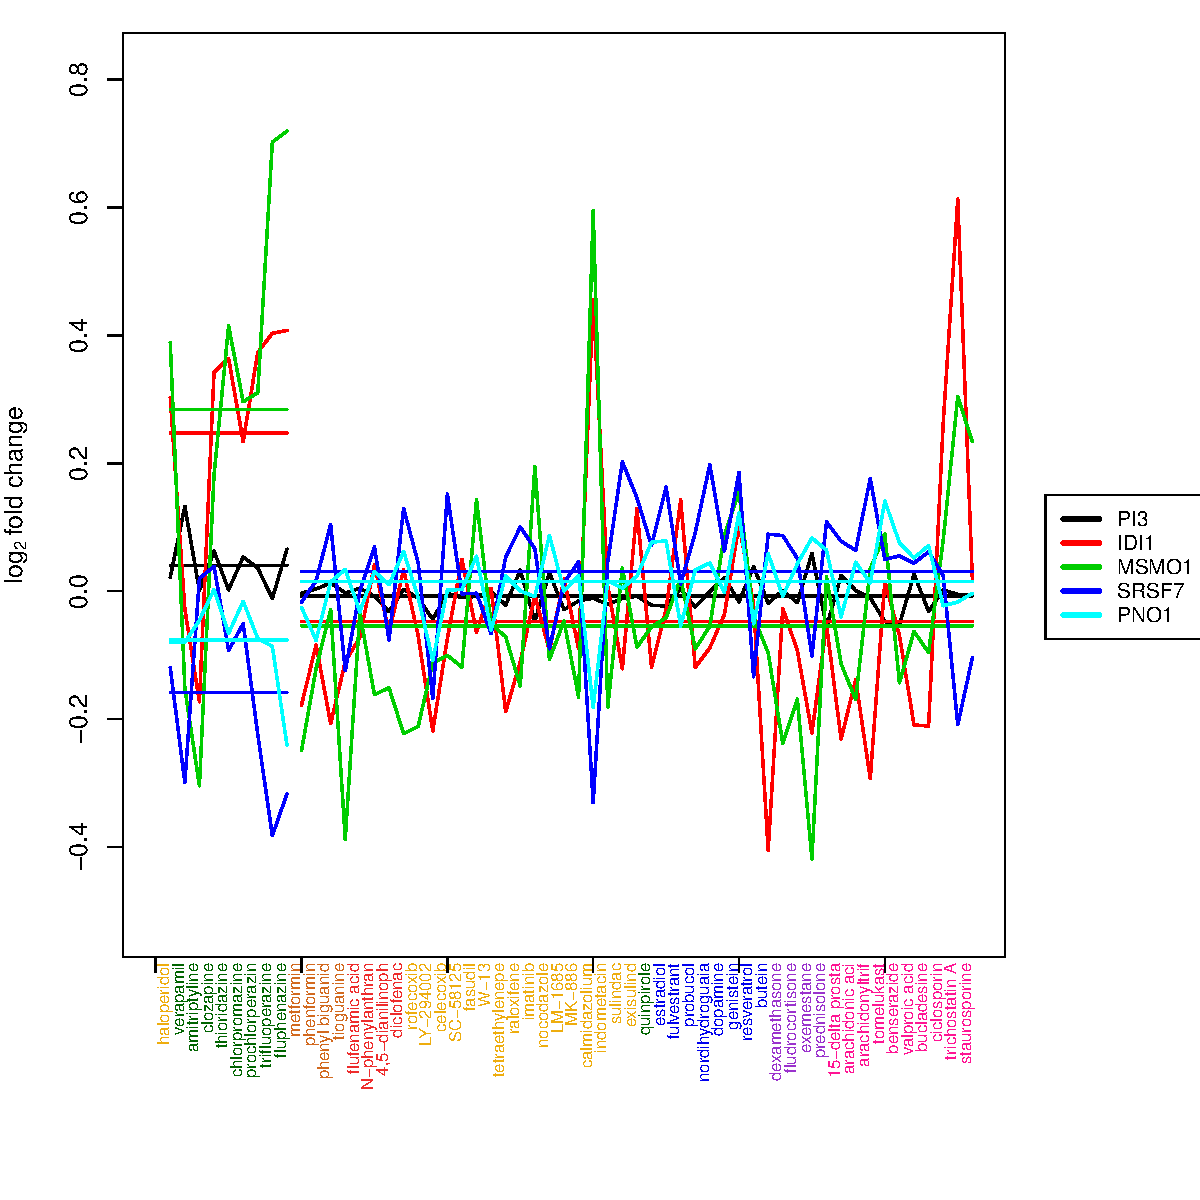
\includegraphics{IntClustVignette-ProfilePlot}
\vspace{-1.0cm}
\caption{{\it The Top $5$ Genes}\label{MCF7_Weights}}
\end{figure}
\newpage
\subsection{Pathway Analysis}
The final step in the analysis is to allocate the genes to a gene set or
pathway. If a gene set is enriched, i.e. the probability to see this many
significant genes of this gene set by chance is low in the selected compounds,
one may be fairly sure that the compounds share an activity on this pathway.
The selected database for pathway analysis is the Gene Ontology (GO) database.
This is an hierarchical database which starts from more general terms
(annotations) to very specific ones. The pathway analysis performed was
functional class scoring, also known as MLP. The search for enriched gene sets
starts from the p-values of all genes. For a predefined gene set, it calculates
a score that summarizes the significance of all the genes included in that
specific set. This score is the mean of the negative logarithm of the p-values
(MLP).\\ \\
It is then determined how likely it is to see the MLP value by chance. This is
done by a comparison with the empirical null distribution. To attain this
distribution, the labels are permuted across the samples and the MLP is
recalculated. This is repeated a few times for all gene sets. The null
distribution of MLP and the observed value of MLP are compared and if there is a
small probability to find the observed MLP (a small p-value for this
distribution), the score is deemed significant. The MLP method to perform
pathway analysis is based on resampling of the data. Therefore it is recommended
to perform the pathway analysis multiple times to observe how much the results
are influenced by a different sample. We will perform iterative pathway analysis
for our selection of compouds with the {\it PathwaySelectionIter} function.
Finally, we will found out how many of these were shared over the different
iterations with the {\it Genseset.intersectSelection} function.
\begin{Schunk}
\begin{Sinput}
> data(GeneInfo)
> data(GS)
> L=list(MCF7_Genes)
> MCF7_Paths=PathwaysIter(List=L,Selection=Comps,names=NULL,
                         GeneExpr=geneMat,nrclusters=7,method=
                         c("limma", "MLP"),GeneInfo=GeneInfo,
                         geneSetSource = "GOBP",topP=NULL,topG=NULL,
                         GENESET=GS,sign=0.05,niter=2,
                         fusionsLog=TRUE,WeightClust=TRUE)
> MCF7_Paths_Inter=Geneset.intersect(MCF7_Paths,Selection=TRUE,sign=0.05,
                                    names=NULL,seperatetables=FALSE,
                                    separatepvals=FALSE)
> 
\end{Sinput}
\end{Schunk}
\newpage
\subsection{Characteristic Features}
It is seen that genes were found to be differential expressed for the selected
compouds which form the green cluster based on target predictions. We could now
investigate whether there are fingerprints or target predictions that define
this cluster. This can be done with the {\it ChooseFeatures} function. The
function has the option to provide the input interactively. A dendrogram of a
provided clustering result will be produces and the user can identify the
cluster of interest by clicking. However, the input can also be provided
manually as we will do now.
\begin{Schunk}
\begin{Sinput}
> MCF7_Feat=ChooseCluster(Interactive=FALSE,LeadCpds=Comps,ClusterResult=MCF7_F,
                         ColorLab=MCF7_F,BinData=list(fingerprintMat,
                         targetMat),Datanames=c("FP","TP"),geneMat,topChar = 20,
                         topG = 20,nrclusters=7,N=1)
\end{Sinput}
\end{Schunk}
\noindent We plot the top identified features with the {\it FeaturesPlot}.
\begin{Schunk}
\begin{Sinput}
> BinFeaturesPlot(LeadCpds=Comps,OrderLab=MCF7_F,Features=
                 MCF7_Feat$Characteristics$FP,Data=fingerprintMat,
                 ColorLab=MCF7_F,nrclusters=7,cols=Colors,name=c("FP"),plottype="sweave",
                 location=NULL)
\end{Sinput}
\end{Schunk}
\begin{Schunk}
\begin{Sinput}
> BinFeaturesPlot(LeadCpds=Comps,OrderLab=MCF7_F,Features=
                 MCF7_Feat$Characteristics$TP,Data=targetMat,ColorLab=MCF7_F,
                 nrclusters=7,cols=Colors,name=c("TP"),plottype="sweave",
                 location=NULL)
\end{Sinput}
\end{Schunk}
\begin{figure}[H]
  \begin{minipage}[b]{.5\linewidth}
     \centering
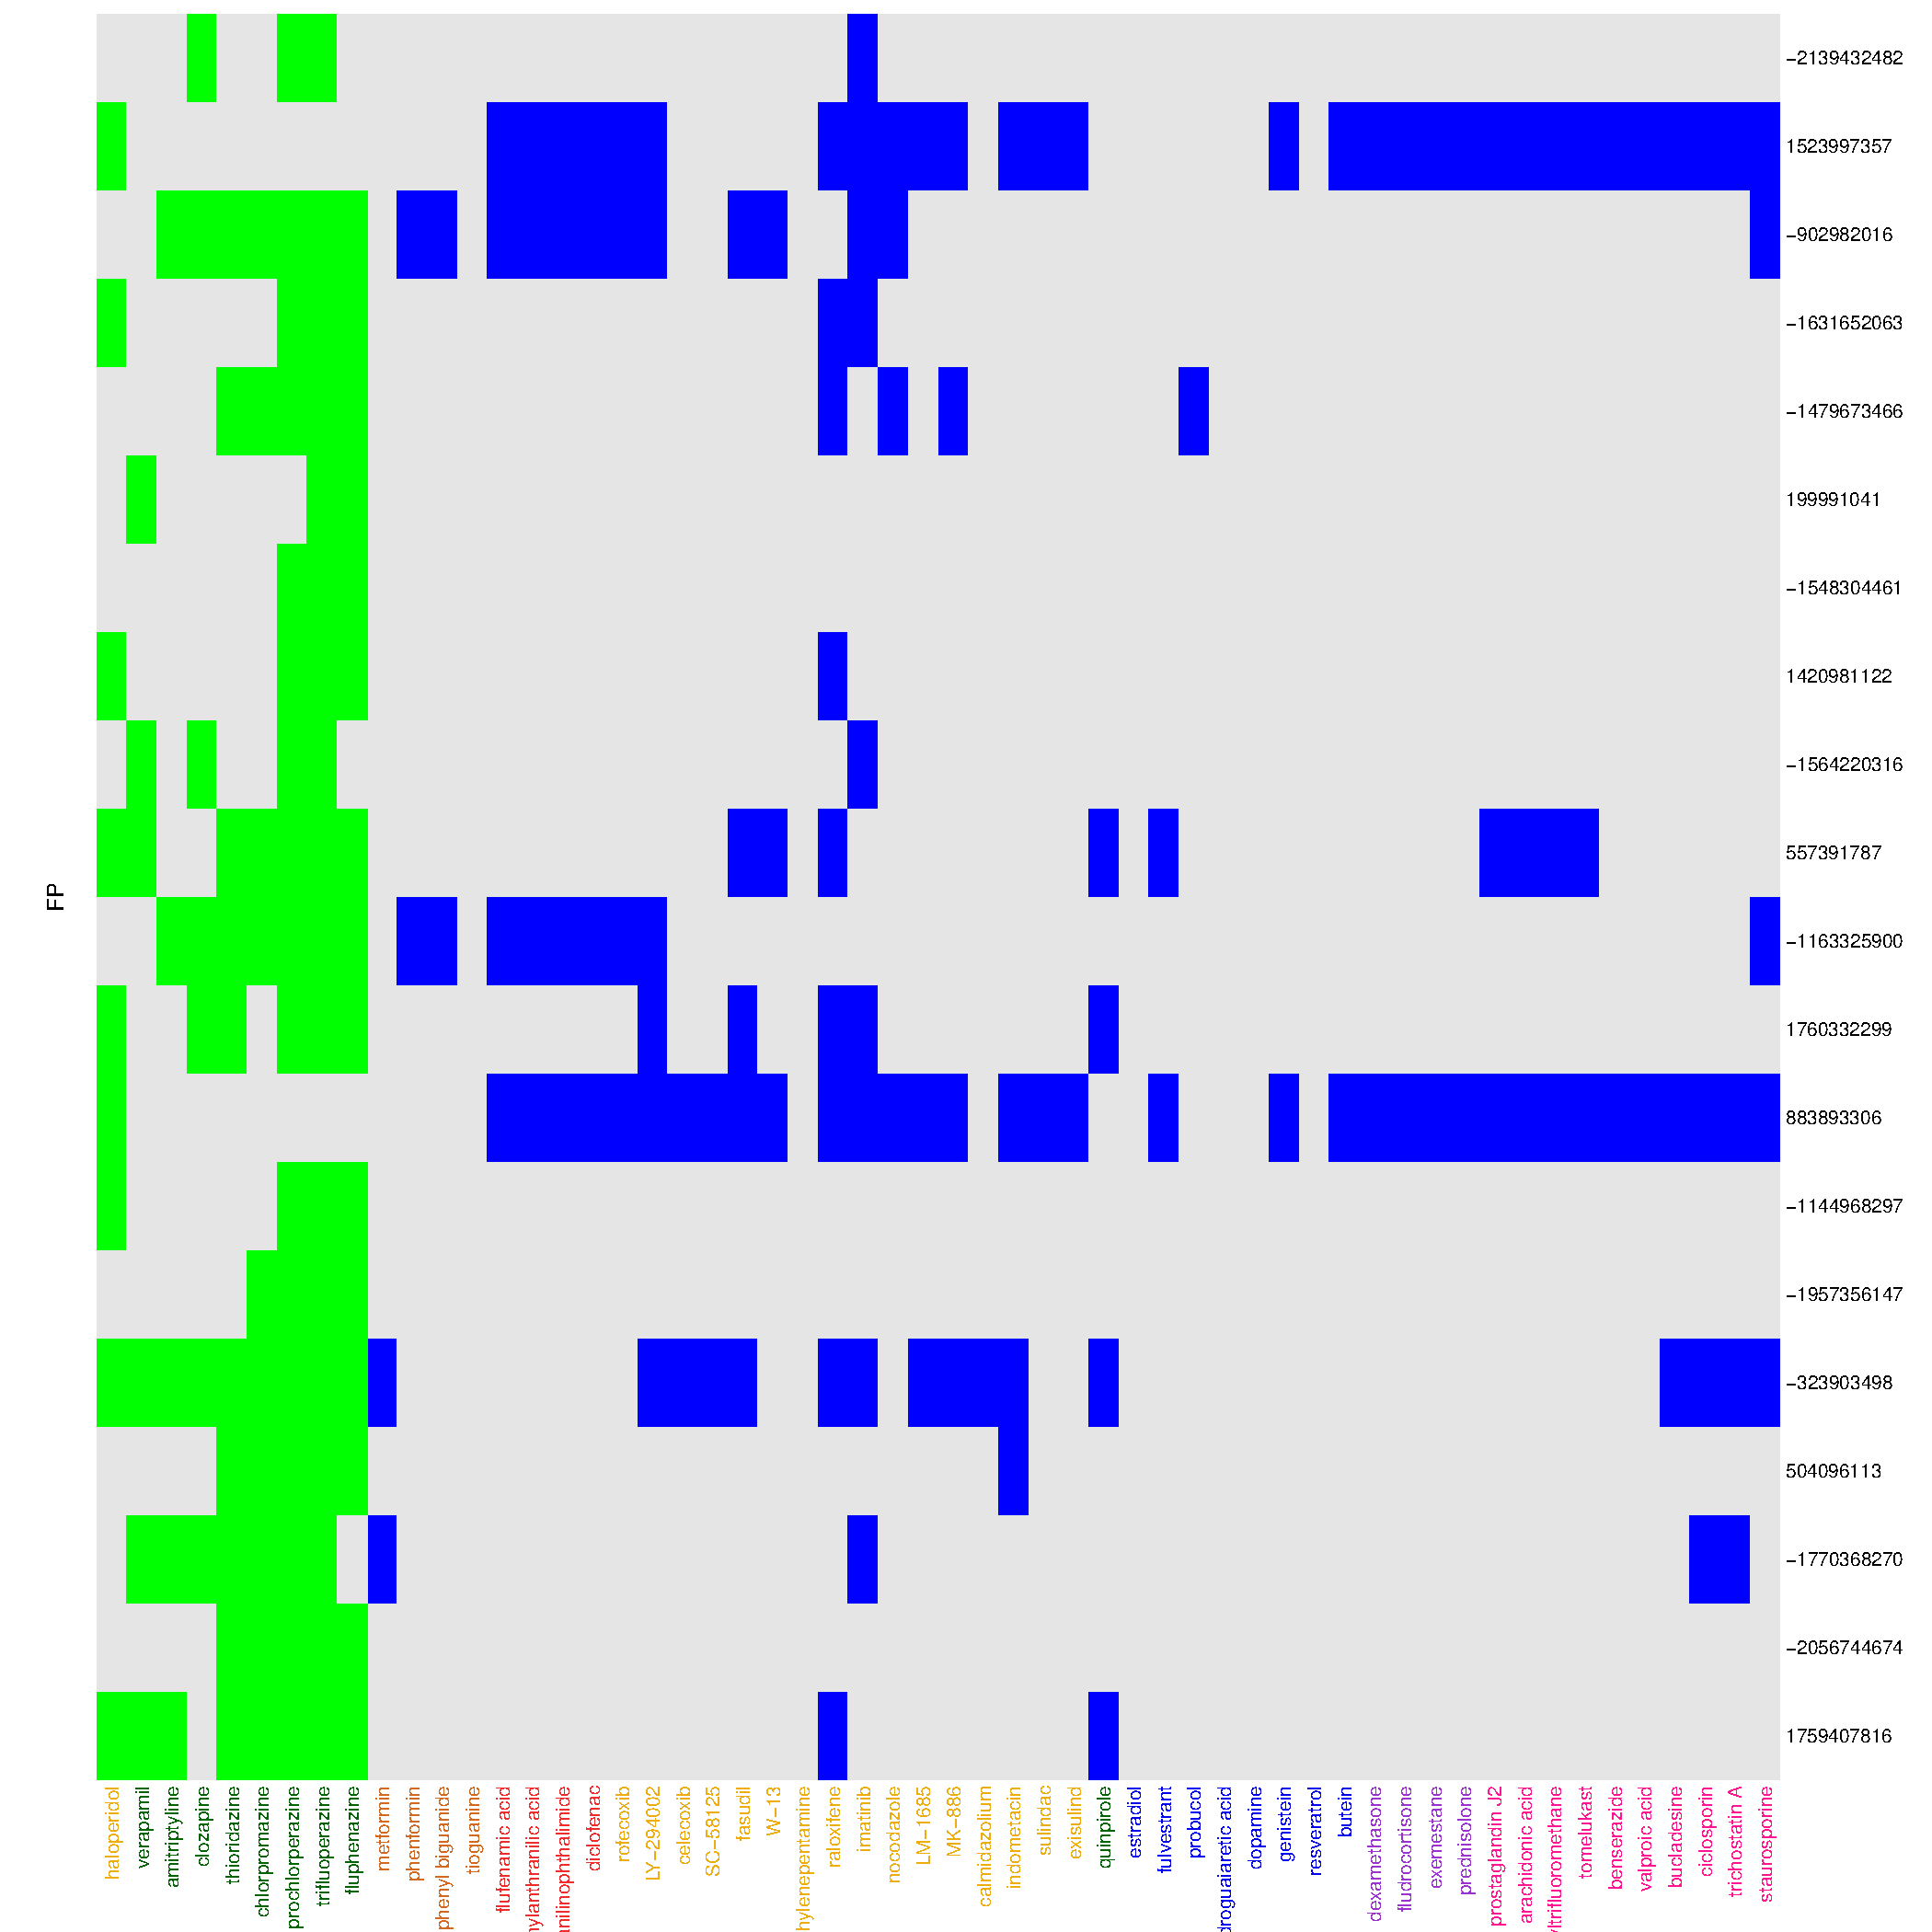
\includegraphics{IntClustVignette-FeaturesPlotFP}
\caption{{\it Top 20 Fingerprints - MCF7}\label{MCF7_F}}
\end{minipage}%
  \begin{minipage}[b]{.5\linewidth}
     \centering
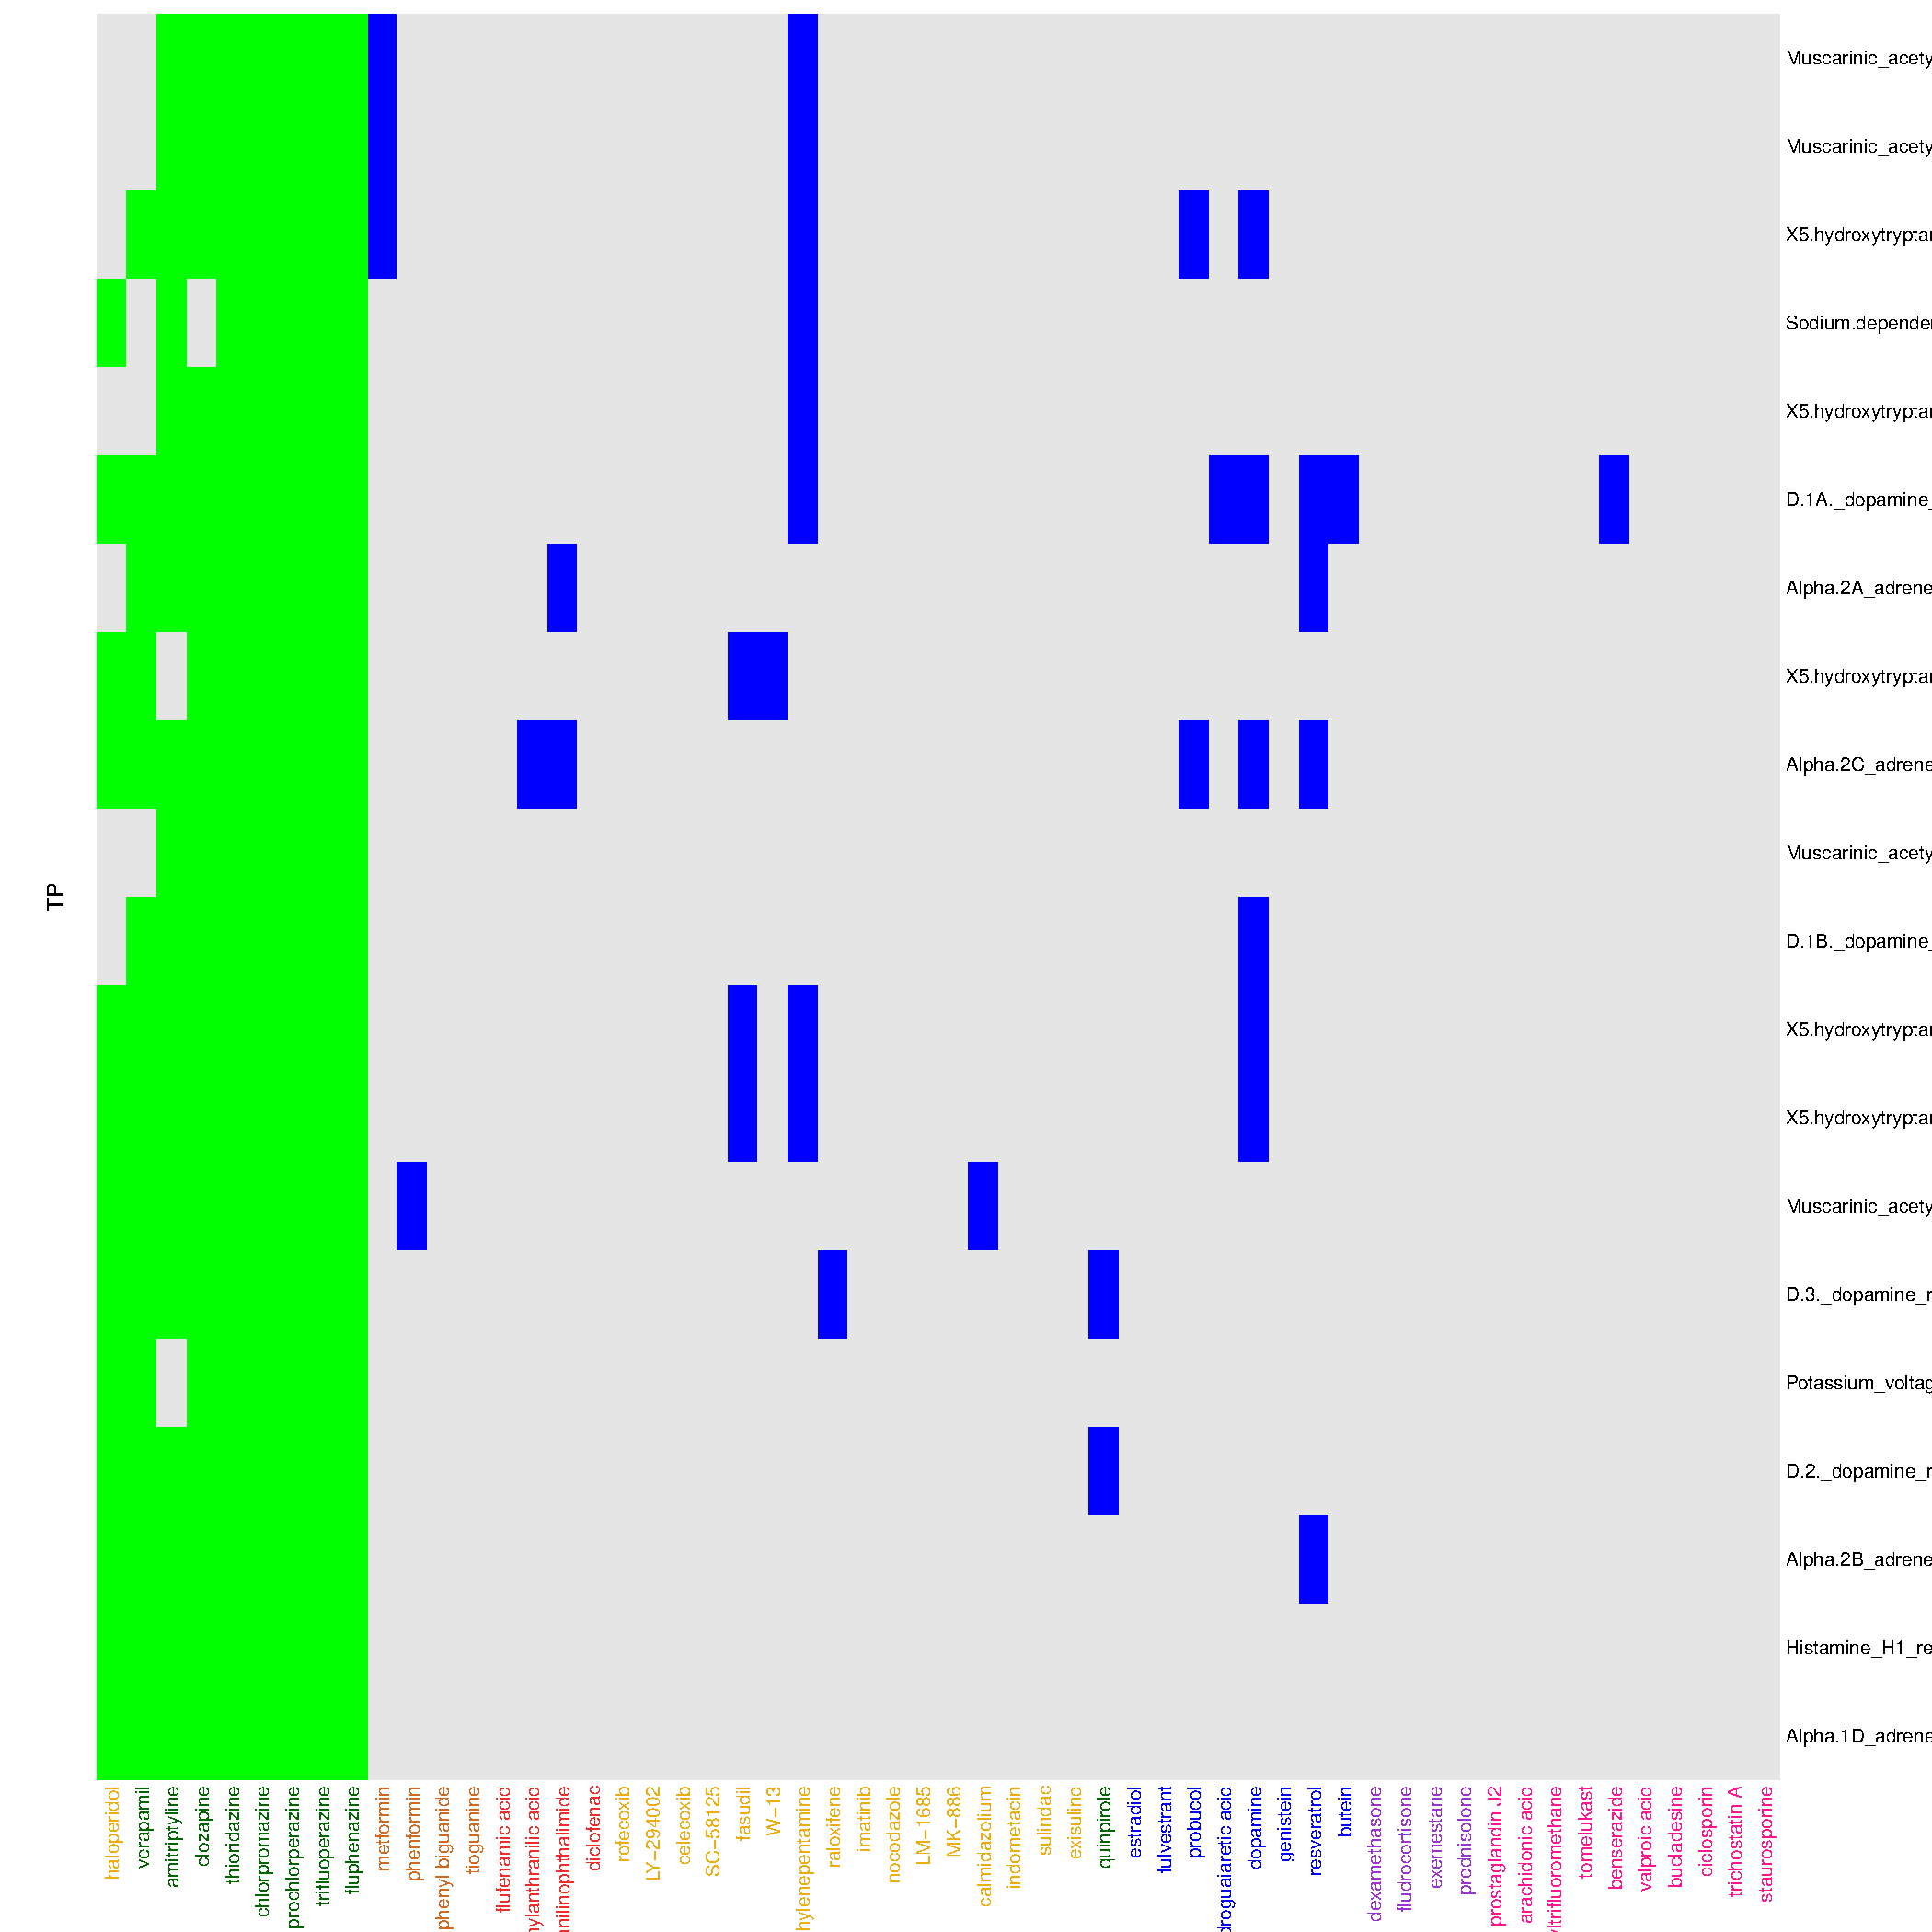
\includegraphics{IntClustVignette-FeaturesPlotT}
\caption{{\it Top 20 target predictions - MCF7}\label{MCF7_F}}
\end{minipage}
\end{figure}
\newpage
\bibliographystyle{asa}
\bibliography{BVSPermbib}
\newpage
\section{Software used}
\begin{itemize}\raggedright
  \item R version 3.1.3 (2015-03-09), \verb|x86_64-w64-mingw32|
  \item Locale: \verb|LC_COLLATE=Dutch_Belgium.1252|, \verb|LC_CTYPE=Dutch_Belgium.1252|, \verb|LC_MONETARY=Dutch_Belgium.1252|, \verb|LC_NUMERIC=C|, \verb|LC_TIME=Dutch_Belgium.1252|
  \item Base packages: base, datasets,
    graphics, grDevices, methods, parallel,
    stats, stats4, tools, utils
  \item Other packages:
    AnnotationDbi~1.28.2, Biobase~2.26.0,
    BiocGenerics~0.12.1, biomaRt~2.22.0,
    DBI~0.3.1, GenomeInfoDb~1.2.5,
    ggplot2~1.0.1, gplots~2.16.0,
    IntClust~0.0.1, IRanges~2.0.1,
    org.Hs.eg.db~3.0.0, rj~2.0.3-1,
    RSQLite~1.0.0, S4Vectors~0.4.0,
    SNFtool~2.2
  \item Loaded via a namespace (and not
    attached): a4Base~1.14.0, a4Core~1.14.0,
    ade4~1.7-2, bitops~1.0-6,
    caTools~1.17.1, class~7.3-12,
    cluster~2.0.1, colorspace~1.2-6,
    digest~0.6.8, e1071~1.6-4, gdata~2.16.1,
    grid~3.1.3, gridExtra~0.9.1,
    gtable~0.1.2, gtools~3.4.2,
    heatmap.plus~1.3, KernSmooth~2.23-14,
    lava~1.4.0, limma~3.22.7, magrittr~1.5,
    MASS~7.3-40, MLP~1.14.0, munsell~0.4.2,
    plotrix~3.5-11, pls~2.4-3, plyr~1.8.2,
    prodlim~1.5.4, proto~0.3-10,
    Rcpp~0.11.6, RCurl~1.95-4.6,
    reshape2~1.4.1, rj.gd~2.0.0-1,
    scales~0.2.4, splines~3.1.3,
    stringi~0.4-1, stringr~1.0.0,
    survival~2.38-1, XML~3.98-1.1
\end{itemize}\end{document}
